\documentclass[11pt,a4paper,twoside]{article}

% ------------------------------------------------------------
% Encoding and Fonts
% ------------------------------------------------------------
\usepackage[utf8]{inputenc}
\usepackage[T1]{fontenc}

% ------------------------------------------------------------
% Math and Symbols
% ------------------------------------------------------------
\usepackage{amsmath,amssymb,amsthm,mathtools}
\usepackage{bm}
\usepackage{physics}

% ------------------------------------------------------------
% Geometry and Layout
% ------------------------------------------------------------
\usepackage{geometry}
\geometry{margin=1in}
\usepackage{setspace}
\setstretch{1.11}

% ------------------------------------------------------------
% Figures, Diagrams, TikZ
% ------------------------------------------------------------
\usepackage{tikz}
\usetikzlibrary{arrows.meta,positioning,decorations.pathreplacing}

% ------------------------------------------------------------
% Hyperlinks
% ------------------------------------------------------------
\usepackage{hyperref}

% ------------------------------------------------------------
% Misc Packages
% ------------------------------------------------------------
\usepackage{enumitem}
\usepackage{parskip}
\usepackage{caption}
\usepackage{booktabs}
\usepackage[
  backend=biber,
  style=authoryear,
  maxbibnames=99
]{biblatex}

\addbibresource{references.bib}


% ------------------------------------------------------------
% Title
% ------------------------------------------------------------
\title{Simulated Agency as Active Control:\\
A Unified Framework Integrating Choice Theory,\\
Perceptual Control Theory, the Free Energy Principle,\\
Sparse Semantic Projection, and Sheaf-Theoretic Coherence}

\author{Flyxion}

\date{November 2025}

\begin{document}

\maketitle

\begin{abstract}
This monograph develops a comprehensive theoretical synthesis unifying
William Glasser’s internal control psychology, William Powers’ Perceptual Control Theory (PCT),
Karl Friston’s Free Energy Principle (FEP), and contemporary sparse-representation
and sheaf-theoretic approaches to cognition.
Although these traditions emerged independently, they converge on a single deep principle:
agents maintain their integrity by minimising a discrepancy functional between an internal normative
model and the sensory world.
This can be achieved only through two operations:
acting on the environment or updating the internal model.
The dual-gradient structure of adaptive behaviour is shown
to be mathematically inevitable given thermodynamic, energetic, and structural constraints.
We formalise these correspondences through variational calculus,
Riemannian geometry, sparse dictionary learning,
and sheaf cohomology, demonstrating that PCT is a special case of active inference
under linear–Gaussian assumptions, that Glasser’s reorganisation corresponds to hyperprior updating,
and that biological sparsity is a thermodynamically inevitable constraint induced by metabolic cost.
The resulting framework provides a unified architecture for
psychology, theoretical neuroscience, and the design of interpretable artificial agents.
\end{abstract}

\newpage

\tableofcontents
\newpage

% ------------------------------------------------------------
% SECTION 1
% ------------------------------------------------------------

\section{Introduction and Motivation}

Across the twentieth century, several intellectual traditions independently converged
on a strikingly similar picture of how agents, organisms, and cognitive systems operate.
William Glasser’s internal control psychology, originating in Reality Therapy
and maturing into Choice Theory \cite{glasser1998choice,glasser1981stations},
conceives behaviour as an internally guided attempt to bring the perceived world
into alignment with an internally constructed ``quality world.''
William T. Powers’ Perceptual Control Theory (PCT)
crystallised these intuitions into a precise cybernetic architecture
\cite{powers1973behavior,powers2005behavior},
asserting that behaviour is not a response to stimuli but the active control of perception.
Half a century later, Karl Friston's Free Energy Principle (FEP)
\cite{friston2009free,friston2010free}
and the associated framework of active inference gave this idea a firm
thermodynamic and Bayesian foundation, describing action and perception as dual aspects
of a single variational imperative: the minimisation of expected surprise.

These traditions—clinical, cybernetic, and mathematical—were not historically connected.
Glasser’s theoretical evolution proceeded largely independently from Powers,
and Powers’ engineering-derived PCT was not directly influenced by Bayesian brain hypotheses.
Nevertheless, their structural forms are astonishingly convergent.
Each views adaptive behaviour as the reduction of a discrepancy between
internal norms and sensory reality.
Each posits two and only two routes for reducing that discrepancy:
altering the world through action, or altering the internal model through learning or reorganisation.
And each, implicitly or explicitly, recognises that persistent error
cannot be resolved within the primary control loop and requires higher-order structural change.

This monograph formalises this convergence.
The early sections trace the psychological and cybernetic roots of control theory,
reconstructing Powers and Glasser with mathematical precision.
Middle sections develop the free-energy formalism, establishing equivalence under linear–Gaussian assumptions,
and introducing sparse semantic projection as an energy-efficient instantiation of internal modelling.
Later sections build a sheaf-theoretic account of perceptual and normative coherence,
demonstrating how conflict corresponds to topological obstruction
and how reorganisation corresponds to global structural repair.
The concluding chapters integrate these into a thermodynamically constrained geometry
of agency, unifying the psychological insights of Glasser and Powers with contemporary theoretical neuroscience.

\newpage

% ------------------------------------------------------------
% SECTION 2
% ------------------------------------------------------------

\section{The Universal Control Duality}

Any autonomous system that persists in a fluctuating environment must regulate its sensory states
relative to internally maintained normative targets.
Regardless of implementation—neural, computational, or mechanical—this requirement leads
to a universal structural form.
Let $\mathcal{M}$ be the space of internal models or normative structures,
$\mathcal{O}$ the space of sensory observations,
and $D(m,o)$ a non-negative discrepancy functional quantifying
the deviation of current observations from the model’s preferred or predicted states.
This functional may be as simple as a quadratic error $(r - p)^2$,
as complex as a variational free energy bound \cite{friston2009free},
or as combinatorial as a mismatch between sparse semantic templates \cite{elad2010sparse,olshausen1996emergence}.

The agent has access to two sets of controllable variables:
actions $a$, which alter the external world or the sensory channel,
and internal parameters $m$, which determine the generative or normative model.
The fundamental duality theorem asserts:

\begin{quote}
\textbf{Universal Control Duality.}
\emph{Minimisation of $D(m,o)$ can occur only through gradient flows in two manifolds:}
\[
\dot{a} \in -\nabla_a \, \mathbb{E}[D(m,o(a))], \qquad
\dot{m} \in -\nabla_m \, D(m,o).
\]
\emph{All adaptive behaviour can be decomposed into these two classes:
changes to the world (action) or changes to the model (learning/reorganisation).}
\end{quote}

This duality is not merely descriptive.
It follows from the geometry of discrepancy minimisation.
If the agent is to preserve its structural and functional identity,
it must confine its trajectories to a subset of states compatible with its survival or competence.
Any deviation creates an error vector field whose negative gradient defines a canonical correction flow.
Control through action adjusts the sensory stream; control through model update
adjusts the predictions or preferences that define the error.

This duality reappears in Glasser’s distinction between ``acting'' and ``reorganising''
\cite{glasser1998choice}, in Powers’ distinction between ``output functions'' and
``reference signals'' \cite{powers1973behavior},
and in Friston’s separation of active and perceptual inference \cite{friston2010free}.
It also reappears in sparse semantic projection,
where the system either selects a better template or updates the sparse dictionary itself.
In sheaf-theoretic terms, it manifests in the need to either change the local section
(perception/action) or alter the gluing data (model structure).

The universal control duality thus serves as the backbone of the unified theory presented here.
Subsequent sections examine how classical and contemporary frameworks instantiate this duality,
and how they differ only in the specifics of their discrepancy functionals and update rules.

\newpage

% ------------------------------------------------------------
% SECTION 3
% ------------------------------------------------------------

\section{Choice Theory and Perceptual Control Theory}

William Glasser’s Choice Theory \cite{glasser1998choice} and William Powers’ Perceptual Control Theory (PCT)
\cite{powers1973behavior,powers2005behavior}
developed in parallel without direct contact for decades, yet they articulate nearly identical
functional architectures of agency.
Both begin with the premise that behaviour is not a reaction to stimuli,
but a means by which an agent maintains its internally valued perceptual conditions.
In Glasser's terms, organisms act so that their perception of the world matches
the contents of their ``quality world,''
a personal internal catalogue of preferred states.
In Powers’ cybernetic formalism, each control unit compares perceived values $p$
to internally specified reference values $r$ and outputs actions that reduce the error $e = r - p$.

\subsection*{3.1 The Standard PCT Loop}

PCT formalises behaviour as an iterated negative-feedback loop.
Let $p = g(o)$ be a perceptual function mapping sensory input to a controlled variable.
A reference signal $r$ specifies the internally desired value.
The loop computes an error
\[
e = r - p,
\]
which is fed into an output function $u = h(e)$ that modulates action $a$,
which in turn alters the environment and thus future observations.

\vspace{1em}

\begin{center}
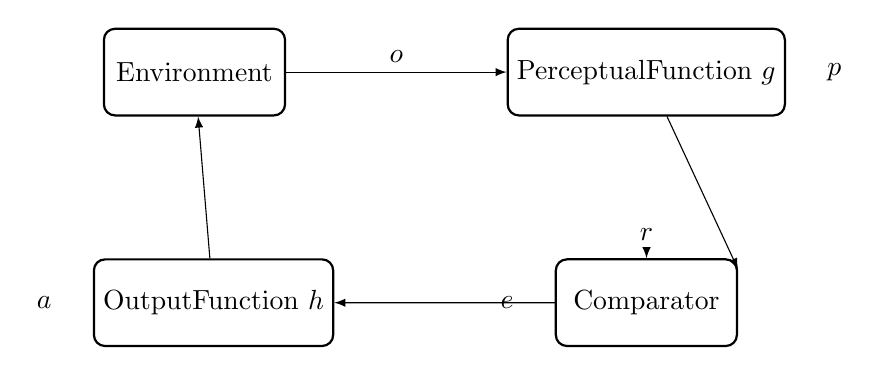
\begin{tikzpicture}[>=latex,scale=1.1]
\tikzstyle{block}=[draw, thick, rectangle, rounded corners, minimum height=1.1cm, minimum width=2.3cm]

\node[block] (env) at (0,0) {Environment};
\node[block, right=2.8cm of env] (per) {Perceptual\\Function $g$};
\node[block, below=1.8cm of per] (cmp) {Comparator};
\node[block, left=2.8cm of cmp] (out) {Output\\Function $h$};

\node[right=0.4cm of per] (p) {$p$};
\node[left=0.4cm of cmp] (e) {$e$};
\node[left=0.4cm of out] (a) {$a$};
\node[above=0.1cm of cmp] (r) {$r$};

\draw[->] (env) -- node[above] {$o$} (per);
\draw[->] (per) -- (cmp.20);
\draw[->] (cmp) -- node[below] {} (out);
\draw[->] (out) -- node[above] {} (env);
\draw[->] (r) -- (cmp);
\end{tikzpicture}

\captionof{figure}{Standard PCT negative-feedback loop.}
\end{center}

\vspace{1em}

Powers argued that nearly all behavioural phenomena—
coordination, conflict, learning, cooperation—emerge from this architecture.
Crucially, PCT reverses the behaviourist stance:
behaviour controls perception, not vice versa.

\subsection*{3.2 Glasser’s Internal Motivation and the Quality World}

Glasser’s theory emphasises internal motivation rather than error correction.
An organism acts to bring life closer to the pictures in its quality world:
belonging, freedom, power, enjoyment.
The behaviour is selected from a ``behavioural system'' in which actions, emotions,
physiology, and cognitions jointly participate in discrepancy reduction.

Glasser’s fundamental insight is categorical:
\emph{behaviour is organised around internal norms, not external stimuli}.
This maps directly to reference signals in PCT and anticipated outcomes in active inference.

\subsection*{3.3 Reorganisation as Second-Order Control}

Powers acknowledged that some errors cannot be corrected within the primary loop.
Persistent error triggers reorganisation:
a slow stochastic parameter-change process aimed at discovering a model configuration
that reduces chronic discrepancy.
Glasser similarly describes ``reorganising'' behavioural systems when chronic frustration persists.

This foreshadows modern active inference’s higher-order hyperparameter updates
\cite{friston2016deep,friston2017}, and that connection is made explicit in later sections.

\subsection*{3.4 Summary}

Both Glasser and Powers recognised that agents do not merely respond to the environment
but actively maintain a preferred relation to it.
Their terminology differs, but the core structure is the same:
a standing norm, a perceived value, their discrepancy, and two possible adjustments:
action or internal change.

These insights anticipated the variational and thermodynamic formulations
of the Free Energy Principle by half a century.
We now turn to that framework.

\newpage

% ------------------------------------------------------------
% SECTION 4
% ------------------------------------------------------------

\section{The Free Energy Principle and Active Inference}

The Free Energy Principle (FEP) developed by Friston
\cite{friston2009free,friston2010free,friston2016deep}
and the associated machinery of active inference offer a rigorous mathematical version
of what Glasser and Powers described qualitatively.
While PCT asserts that behaviour controls perception,
FEP proposes that perception and action jointly minimise a variational free energy bound
on surprise or self-inconsistency.
Thus, both frameworks posit a coupled pair of gradient flows in the space of actions and beliefs.

\subsection*{4.1 Generative Models and Bayesian Inference}

An agent maintains a generative model of sensory states.
Let $o$ denote observations and $s$ hidden causes.
The model factorises as:
\[
p(o,s\mid m) = p(o\mid s,m)\,p(s\mid m),
\]
where $m$ are model parameters (priors, precisions, structural assumptions).
Inverting this model yields the posterior:
\[
p(s\mid o,m) = \frac{p(o,s\mid m)}{p(o\mid m)}.
\]

\subsection*{4.2 Variational Free Energy}

Exact inference is often intractable, so the agent uses an approximate posterior $q(s)$.
Variational inference chooses $q$ to minimise:
\[
\mathrm{KL}[q(s)\|p(s\mid o,m)].
\]
Because $\ln p(o)$ is constant with respect to $q$,
we obtain the variational identity:
\[
\ln p(o) = F[q] + \mathrm{KL}[q\|p(s\mid o)],
\]
where
\[
F[q] = \mathbb{E}_q[\ln q(s)] - \mathbb{E}_q[\ln p(o,s)].
\]

Thus minimising $F$ minimises an upper bound on surprise.

\subsection*{4.3 Accuracy–Complexity Trade-off}

Free energy decomposes into:
\[
F = \underbrace{\mathrm{KL}[q(s)\|p(s)]}_{\text{complexity}}
    - \underbrace{\mathbb{E}_q[\ln p(o\mid s)]}_{\text{accuracy}}.
\]
This recovers Glasser’s idea that the brain balances fidelity to evidence
against maintaining a stable quality world.

\subsection*{4.4 Dual Gradient Flows}

Active and perceptual inference follow:
\[
\dot{\mu} = -\partial_\mu F, \qquad
\dot{a} = -\partial_a F.
\]
The second expression expands via the sensory mapping $o(o(a))$:
\[
\partial_a F = \frac{\partial F}{\partial o}\frac{\partial o}{\partial a}.
\]

This is the mathematical version of Powers’ loop.

\subsection*{4.5 Expected Free Energy and Policies}

For temporally extended behaviour,
agents minimise expected free energy:
\[
G(\pi) = \mathbb{E}_{q(o_\tau,s_\tau|\pi)}[F].
\]
$G$ decomposes into expected ambiguity (epistemic value)
and expected deviation from goals (pragmatic value)
\cite{friston2016deep,brown2013active}.

In environments where epistemic value is negligible,
PCT’s pure control of perception is recovered exactly.

\subsection*{4.6 Nonequilibrium Thermodynamics}

Organisms exist in nonequilibrium steady states.
The FEP formalises adaptive behaviour as keeping system trajectories on low-surprisal
attractors in state space.

This also provides the thermodynamic grounding missing in classical cybernetics
\cite{sengupta2016}.

\subsection*{4.7 Preferences as Priors}

In FEP, preferences are priors over sensory states:
\[
p(o) \propto \exp\!\left(-\frac{(o-r)^2}{2\sigma_r^2}\right),
\]
making reference signals explicit probabilistic objects.

\subsection*{4.8 Hierarchical Models and PCT Levels}

Generative models naturally stack into hierarchies \cite{hohwy2013},
mirroring the layered organisation of PCT’s perceptual and control structure.

\subsection*{4.9 Learning and Structure}

Parameters and hyperparameters are updated via:
\[
\dot{m} = -\eta\,\partial_m F.
\]
This is precisely Powers’ ``reorganisation'' and Glasser’s ``new behaviour selection.''

\subsection*{4.10 Summary}

FEP provides a mathematically rigorous account of the same functional architecture
proposed by PCT and Choice Theory.
Section~5 develops this equivalence explicitly.

\newpage

% ------------------------------------------------------------
% SECTION 5
% ------------------------------------------------------------

\section{Formal Equivalence of PCT and Active Inference}

The convergence between Perceptual Control Theory (PCT) and the Free Energy Principle (FEP)
is not merely metaphorical.
Despite originating in separate intellectual lineages—cybernetics and control theory in the case of Powers
\cite{powers1973behavior,powers2005behavior},
and statistical physics, variational inference, and theoretical neuroscience in the case of Friston
\cite{friston2009free,friston2010free}—
both frameworks describe organisms as systems that regulate their sensory trajectories
relative to internally preferred states.
This section establishes a formal equivalence theorem:
under linear-Gaussian assumptions, the PCT control loop is exactly the special case
of active inference in which expected free energy reduces to pragmatic (goal-directed) error.

\subsection*{5.1 PCT Control Law as a Gradient Flow}

Let $p$ be a scalar or vector perceptual variable,
and let the agent stipulate a reference value $r$.
PCT defines the behavioural loop as:
\[
e = r - p, \qquad
a = h(e),
\]
where $h$ is a gain (linear or nonlinear) mapping discrepancy into motor output.
Assuming a linear output function,
\[
a = k \, (r - p),
\]
and assuming perception depends differentiably on action,
\[
p = g(o(a)),
\]
the closed-loop dynamics become:
\[
\dot{a} = k \left( r - g(o(a)) \right).
\]

Thus PCT prescribes a gradient flow that reduces the discrepancy $r - p$.

\subsection*{5.2 Active Inference Control Law}

Active inference expresses action as a gradient of variational free energy:
\[
\dot{a} = -\frac{\partial F}{\partial a}
       = -\frac{\partial F}{\partial o}\frac{\partial o}{\partial a}.
\]
Under a Gaussian likelihood with desired mean $r$ and sensory mapping $o(s)$:
\[
p(o\mid s) \propto \exp\!\left(
 -\frac{(o-r)^2}{2\sigma_r^2}
\right),
\]
the accuracy term of the free energy is:
\[
\mathbb{E}_q[(o - r)^2].
\]
Thus the action-gradient becomes:
\[
\dot{a} = \frac{1}{\sigma_r^2}
          (o - r)\frac{\partial o}{\partial a}
        = -k (r - o)\frac{\partial o}{\partial a},
\]
where $k = \sigma_r^{-2}$.

This is exactly a PCT error-minimisation law with an additional Jacobian term.

\subsection*{5.3 The Jacobian Term and Effective Gain}

Powers assumed a direct causal pathway from action to perception:
\[
a \rightarrow \text{environment} \rightarrow o \rightarrow g \rightarrow p.
\]
Active inference formalises this causal chain with an explicit derivative:
\[
\frac{\partial o}{\partial a}.
\]
Thus PCT’s gain $k$ corresponds to an \emph{effective} gain:
\[
k_{\text{eff}} = k \,\frac{\partial o}{\partial a}.
\]
When $\partial o/\partial a$ is constant or approximated as unity,
PCT and active inference produce identical trajectories in action space.

\subsection*{5.4 The Equivalence Theorem}

\begin{theorem}[Equivalence of PCT Control and Pragmatic Active Inference]
Let the generative model be linear-Gaussian in both dynamics and observation.
Assume preferences are encoded as Gaussian priors over sensory states with mean $r$.
Assume epistemic value is negligible (e.g.\ no uncertainty about hidden causes).
Then the active inference action update reduces to the PCT control law.
\end{theorem}

\begin{proof}
Under the stated assumptions, the free energy reduces to the accuracy term:
\[
F = \frac{1}{2\sigma_r^2}(o-r)^2 + \text{const}.
\]
Taking the action derivative:
\[
\frac{\partial F}{\partial a}
= \frac{1}{\sigma_r^2}(o-r)\frac{\partial o}{\partial a}.
\]
Thus:
\[
\dot{a} = -\frac{\partial F}{\partial a}
= k(r - o)\frac{\partial o}{\partial a}.
\]
If $\partial o/\partial a = 1$ or is absorbed into the gain constant, then:
\[
\dot{a} = k(r - o),
\]
which is the PCT law.
\end{proof}

\subsection*{5.5 Diagrammatic Equivalence}

\vspace{1em}
\begin{center}
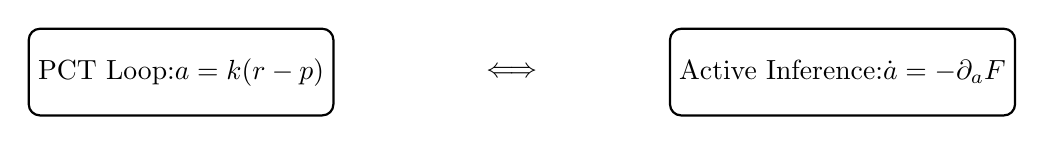
\begin{tikzpicture}[>=latex,scale=1.05]
\tikzstyle{block}=[draw, thick, rectangle, rounded corners, minimum height=1.1cm, minimum width=2.5cm]

% PCT block
\node[block] (pct) at (0,0) {PCT Loop:\\$a = k(r - p)$};

% arrow
\node at (4,0) {$\Longleftrightarrow$};

% Active inference block
\node[block] (ai) at (8,0) {Active Inference:\\$\dot{a} = -\partial_a F$};

\end{tikzpicture}

\captionof{figure}{Equivalence of the PCT control law and the pragmatic active inference law under linear-Gaussian assumptions.}
\end{center}
\vspace{1em}

\subsection*{5.6 Interpretation}

The theorem demonstrates that PCT and active inference describe the same mechanism
at different levels of mathematical generality.
PCT corresponds to a free-energy-minimising agent with:

\begin{itemize}
    \item no epistemic drive,
    \item direct sensory control,
    \item a fixed-point preference distribution,
    \item and a single-level generative model.
\end{itemize}

Conversely, active inference offers:

\begin{itemize}
    \item hierarchical perception,
    \item explicit uncertainty quantification,
    \item epistemic action,
    \item and nonequilibrium thermodynamic grounding.
\end{itemize}

Thus PCT is the \emph{non-epistemic, single-level special case} of active inference.

\subsection*{5.7 Consequences}

This equivalence has three major consequences for cognitive science:

\begin{enumerate}
    \item Glasser’s quality world and Powers’ reference values become preference priors.
    \item Behavioural reorganisation becomes hyperparameter optimisation.
    \item Persistent psychological conflict becomes a case of incompatible priors,
          or competing control loops with shared environmental variables.
\end{enumerate}

These interpretations motivate the clinical applications developed later in the paper.

\newpage

% ------------------------------------------------------------
% SECTION 6
% ------------------------------------------------------------

\section{Hierarchy, Conflict, and Internal Models}

The equivalence established in the previous section clarifies that perceptual control
and active inference share a common functional architecture.
However, living systems are not single-loop regulators.
They organise perception and action into hierarchies of increasing temporal depth,
spatial generality, and semantic abstraction.
This was emphasised by Powers in his hierarchical model
\cite{powers1973behavior,powers2005behavior},
by Glasser through his tiered descriptions of needs, pictures, and total behaviour
\cite{glasser1981stations,glasser1998choice},
and by Friston in hierarchical generative models of cortical function
\cite{friston2009free,friston2010free}.

This section formalises the hierarchical architecture of adaptive control systems,
derives its stability conditions, and provides a unified interpretation of psychological
conflict in the language of both PCT and the Free Energy Principle.
Where Section~5 addressed the equivalence of the *single loop*, this section extends the analysis to multilayer control and inference.

\subsection*{6.1 Hierarchical Perceptual Functions}

In Powers’ original formulation, perceptual variables $p^{(l)}$ at level $l$ are constructed as
functions of variables at the level below:
\[
p^{(l)} = f^{(l)}\!\left(p^{(l-1)}\right),
\qquad l = 1,2,\ldots,L,
\]
where $p^{(0)}$ corresponds to unprocessed sensory input.

In hierarchical active inference, the equivalent expression is the factorisation of the generative model:
\[
p(o,s^{(1)},\ldots,s^{(L)})
= p(o \mid s^{(1)})
\prod_{l=1}^{L} p(s^{(l)} \mid s^{(l+1)}),
\]
with the convention that $s^{(L+1)}$ is a hyperprior or context state.

The mapping
\[
p^{(l)} \leftrightarrow \mathbb{E}[s^{(l)}]
\]
is the formal equivalence between hierarchical perceptual functions and hierarchical latent variables.

\subsection*{6.2 Error Propagation and Predictive Coding}

For each hierarchical level, Powers described error signals as:
\[
e^{(l)} = r^{(l)} - p^{(l)}.
\]
In active inference, hierarchical prediction error is:
\[
\varepsilon^{(l)} =
\Sigma_l^{-1}\left(s^{(l)} - g^{(l)}(s^{(l+1)})\right),
\]
where $\Sigma_l$ encodes precision.

The equivalence is:
\[
e^{(l)} \leftrightarrow \varepsilon^{(l)}.
\]

Where PCT emphasises discrepancies relative to reference values $r^{(l)}$,
active inference expresses these as priors over causes.

\subsection*{6.3 The Stability Condition for Hierarchical Control}

Hierarchical control requires that lower-level loops operate more rapidly than higher ones.
Powers stressed that a higher loop *sets* the reference for the lower loop but must not interfere with its rapid dynamics.

This is formalised by the timescale ordering:
\[
\tau_0 \ll \tau_1 \ll \tau_2 \ll \cdots \ll \tau_L.
\]

Mathematically, consider a two-level system:
\[
\begin{aligned}
\dot{a} &= k_0 (r^{(0)} - p^{(0)}), \\
\dot{r}^{(0)} &= k_1 (r^{(1)} - p^{(1)}),
\end{aligned}
\]
with $p^{(1)} = f(p^{(0)})$.

Linearising around equilibrium yields:
\[
\begin{pmatrix}
\dot{a} \\
\dot{r}^{(0)}
\end{pmatrix}
=
\begin{pmatrix}
-k_0 \frac{\partial p^{(0)}}{\partial a} & k_0 \\
-k_1 \frac{\partial p^{(1)}}{\partial p^{(0)}}\frac{\partial p^{(0)}}{\partial a} &
 -k_1 \frac{\partial p^{(1)}}{\partial r^{(0)}}
\end{pmatrix}
\begin{pmatrix}
a \\
r^{(0)}
\end{pmatrix}.
\]

The system is stable if the eigenvalues of the Jacobian have negative real parts.
Sufficient conditions:
\[
k_1 \ll k_0, \qquad
\left|\frac{\partial p^{(1)}}{\partial p^{(0)}}\right|
\ll
\left|\frac{\partial p^{(0)}}{\partial a}\right|.
\]

These are precisely the conditions Powers articulated informally.

\subsection*{6.4 Conflict as Misaligned Reference Priors}

Powers defined conflict as the case where two control systems attempt to regulate the same perceptual variable to incompatible reference values.
Formally, let two loops attempt to control $p$:
\[
\dot{a}_1 = k_1(r_1 - p), \qquad
\dot{a}_2 = k_2(r_2 - p),
\]
with the joint effect on $p$ given by $a = a_1 + a_2$.

If $r_1 \neq r_2$ and the system cannot satisfy both, then the equilibrium
\[
p^\ast = \frac{k_1 r_1 + k_2 r_2}{k_1 + k_2}
\]
fails to satisfy the goal of either loop.

In active inference, reference values are priors:
\[
p(o) \sim \mathcal{N}(r_1,\sigma_1^2),
\qquad
p(o) \sim \mathcal{N}(r_2,\sigma_2^2).
\]

Conflict is expressed as incompatible preferences,
or equivalently as:
\[
\text{No joint prior } p(o) \text{ satisfying both } r_1 \text{ and } r_2.
\]

The free energy surface develops a saddle or ridge, preventing joint minimisation.

\subsection*{6.5 Diagram: Hierarchical Control vs Generative Hierarchy}

\begin{center}
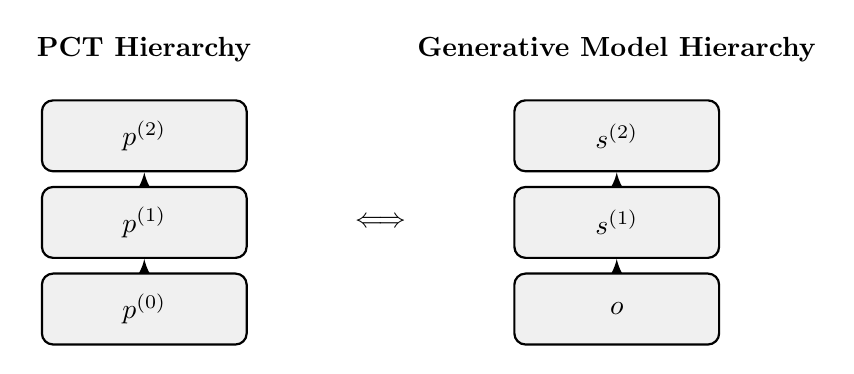
\begin{tikzpicture}[>=latex,scale=1]
\tikzstyle{lvl}=[draw, thick, rectangle, rounded corners,
minimum height=0.9cm, minimum width=2.6cm, fill=gray!12]

% PCT hierarchy
\node at (0,2.8) {\textbf{PCT Hierarchy}};
\node[lvl] (pct3) at (0,1.7) {$p^{(2)}$};
\node[lvl] (pct2) at (0,0.6) {$p^{(1)}$};
\node[lvl] (pct1) at (0,-0.5) {$p^{(0)}$};

\draw[->,thick] (pct1) -- (pct2);
\draw[->,thick] (pct2) -- (pct3);

% Active inference
\node at (6,2.8) {\textbf{Generative Model Hierarchy}};
\node[lvl] (ai3) at (6,1.7) {$s^{(2)}$};
\node[lvl] (ai2) at (6,0.6) {$s^{(1)}$};
\node[lvl] (ai1) at (6,-0.5) {$o$};

\draw[->,thick] (ai1) -- (ai2);
\draw[->,thick] (ai2) -- (ai3);

% arrow between hierarchies
\node at (3,0.6) {$\Longleftrightarrow$};

\end{tikzpicture}

\captionof{figure}{Diagrammatic equivalence of Powers’ perceptual hierarchy and Friston’s hierarchical generative model.}
\end{center}

\subsection*{6.6 Psychological Interpretation}

\paragraph{Glasser’s Quality World.}
Glasser described the “quality world” as an internal set of desired perceptions,
pictures of the life one wants
\cite{glasser1981stations,glasser1998choice}.
This corresponds directly to a hierarchy of preference priors.

\paragraph{Powers’ Conflict.}
Powers insisted that almost all psychological distress emerges from conflict between control systems.
In active inference, this is expressed as incompatible priors or competing modes of a generative model.

\paragraph{Friston’s Nonequilibrium Steady-State Maintenance.}
Friston’s account completes the picture by embedding the hierarchy within a thermodynamic framework:
living systems maintain themselves by minimising the variational free energy associated with their sensory flows
\cite{friston2009free,friston2010free,friston2013life}.

\subsection*{6.7 Summary}

Hierarchical organisation is not an optional feature of adaptive agency.
It is a mathematically necessary architecture for stability, flexibility, and complexity.
The alignment between PCT, Choice Theory, and the Free Energy Principle becomes especially clear at the hierarchical level:

\begin{itemize}
    \item Powers provides the structural hierarchy.
    \item Glasser provides the motivational hierarchy (quality world and basic needs).
    \item Friston provides the probabilistic and thermodynamic hierarchy.
\end{itemize}

These perspectives converge into a single unified model, preparing the way for Section~7,
which develops the explicit sheaf-theoretic representation of hierarchical control.

\section{Sheaf-Theoretic Unification of Hierarchical Control}

Sheaf theory provides a formal language for describing how local pieces of information combine to form coherent global structures. This property makes it uniquely well suited for modelling hierarchical perceptual control, where an agent must reconcile heterogeneous, context-dependent percepts with an internally coherent ``reference world.'' Drawing on the classical foundations of Bredon~\cite{bredon1997sheaf}, the applied compositionality program of Spivak and Fong~\cite{spivak2014category,fong2019invitation}, and recent sheaf-theoretic proposals in cognitive science and signal processing~\cite{curry2021sheafcomp,iverson2021sheaflearning,glazebrook2022,robinson2023sheaf}, this section introduces a rigorous sheaf-theoretic formulation of PCT, Choice Theory, and active inference.

The core thesis is that the \emph{perceptual hierarchy is a sheaf}, the \emph{reference hierarchy is another sheaf}, and \emph{psychological stability corresponds to the existence of global sections whose discrepancies vanish under a morphism between them}. Conversely, persistent psychological conflict corresponds to a failure of the gluing axioms, expressible as a \v{C}ech cohomology obstruction.

This sheaf-theoretic view explains, with mathematical precision, how local perceptual updates (e.g., from contradictory sensory cues or relationship conflicts) may remain irreconcilable at a global scale---precisely the class of problems that PCT characterises as chronic error and Glasser identifies with relationship pathologies, and which active inference formalises as persistent free-energy gradients.

\subsection{7.1 Preliminaries: Contexts, Covers, and Presheaves}

Let $X$ denote the agent's contextual space, whose points correspond to situations, modalities, or task contexts. A \emph{cover} $\mathcal{U}={U_i}$ represents the set of contexts relevant for the agent (e.g., social situations, interoceptive states, goals, tasks).

A \emph{presheaf} $\mathcal{F}$ on $X$ assigns:
\begin{itemize}
\item to each context $U_i$ a set (or vector space) $\mathcal{F}(U_i)$ of perceptual representations, and
\item to each inclusion $V\subseteq U$ a restriction map $\rho_{U V}:\mathcal{F}(U)\to\mathcal{F}(V)$.
\end{itemize}

Intuitively, $\mathcal{F}(U)$ is ``what the agent perceives when attending to context $U$,'' while $\rho_{UV}$ formalises the compatibility between broader and more specific contexts.

A \emph{section} $s\in\mathcal{F}(U)$ represents a perceptual estimate in that context.

Following Spivak~\cite{spivak2013ologs}, a presheaf expresses all local percepts, but not yet their global consistency.

\subsection{7.2 Perception and Reference as Sheaves}

The perceptual hierarchy of PCT can be directly represented as a sheaf:
[
\mathcal{P}: X^{op}\to\mathbf{Set}, \qquad U\mapsto \mathcal{P}(U).
]
Similarly, the \emph{Quality World} or system of internal reference values in Choice Theory becomes another sheaf:
[
\mathcal{R}: X^{op}\to\mathbf{Set}.
]

A \emph{sheaf morphism} (natural transformation)
[
\Phi: \mathcal{P} \Rightarrow \mathcal{R}
]
assigns to every context a perceptual-to-reference comparison map, generalising Powers's error signal and Friston's preference divergence.

\begin{figure}[h]
\centering
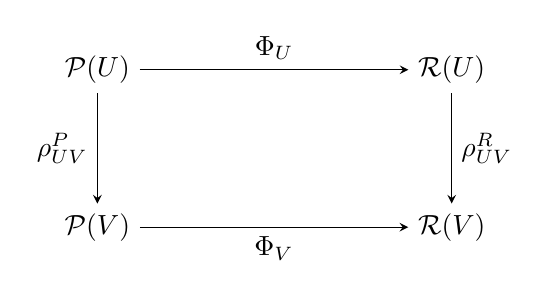
\begin{tikzpicture}[node distance=2cm,>=stealth]
\node (PU) {$\mathcal{P}(U)$};
\node (PV) [below of=PU] {$\mathcal{P}(V)$};
\node (RU) [right of=PU, xshift=2.5cm] {$\mathcal{R}(U)$};
\node (RV) [below of=RU] {$\mathcal{R}(V)$};

\draw[->] (PU) -- node[left] {$\rho^P_{UV}$} (PV);
\draw[->] (RU) -- node[right] {$\rho^R_{UV}$} (RV);
\draw[->] (PU) -- node[above] {$\Phi_U$} (RU);
\draw[->] (PV) -- node[below] {$\Phi_V$} (RV);
\end{tikzpicture}
\caption{A commutative square expressing compatibility of percept--reference comparisons across contexts.}
\end{figure}

Commutativity of the square enforces that perceptual discrepancy measured in a coarse context agrees with the discrepancy measured in a refined one---this is the sheaf-theoretic version of hierarchical consistency in PCT.

\subsection{7.3 Gluing and Global Consistency}

A family of sections ${s_i\in\mathcal{P}(U_i)}$ is \emph{compatible} if their restrictions agree on overlaps:
[
\rho^P_{U_i,U_i\cap U_j}(s_i)
=============================

\rho^P_{U_j,U_i\cap U_j}(s_j).
]

If compatible families always glue uniquely to a global section $s\in\mathcal{P}(X)$, then $\mathcal{P}$ is a sheaf.

By analogy:
[
\text{psychological stability}
\iff
\exists s \in \Gamma(X,\mathcal{P}) \text{ such that } \Phi(s)=r
]
for some desired global reference $r \in \Gamma(X,\mathcal{R})$.

This is aligned with:
\begin{itemize}
\item Powers’s requirement for higher-order control: global consistency across perceptual levels.
\item Glasser’s requirement for relationship coherence in the Quality World.
\item Active inference's requirement that a single $q(s)$ minimize free energy across sensory modalities.
\end{itemize}

\subsection{7.4 \v{C}ech Cohomology and Psychological Conflict}

Failures of gluing appear as \v{C}ech cohomology classes:
[
\check{H}^1(X,\mathcal{P}) \neq 0.
]

In cognitive terms:

\begin{itemize}
\item A \emph{cohomological obstruction} corresponds to incompatible perceptions across contexts.
\item These manifest as persistent error signals in PCT.
\item In Choice Theory they appear as chronic relationship conflicts.
\item In active inference they correspond to free-energy minima that cannot be simultaneously realised.
\end{itemize}

\begin{figure}[h]
\centering
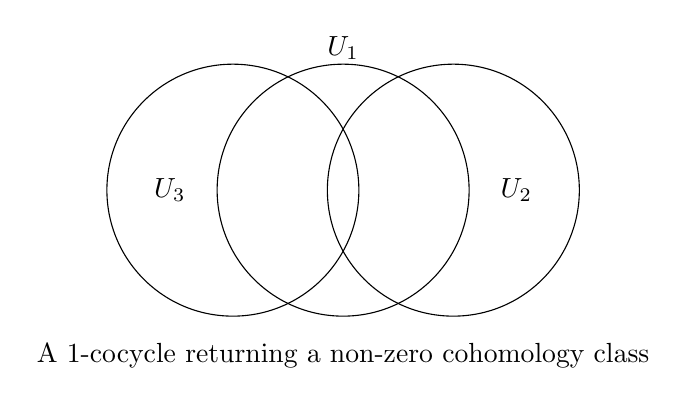
\begin{tikzpicture}[>=stealth]
\draw (0,0) circle (1.6cm);
\draw (1.4,0) circle (1.6cm);
\draw (-1.4,0) circle (1.6cm);

\node at (0,1.8) {$U_1$};
\node at (2.2,0) {$U_2$};
\node at (-2.2,0) {$U_3$};

\node at (0,-2.1) {A 1-cocycle returning a non-zero cohomology class};
\end{tikzpicture}
\caption{A cycle of contexts whose perceptual overlaps contain an inconsistency that cannot be globally resolved. Psychological conflict corresponds to non-trivial cycles.}
\end{figure}

This diagram represents a loop of perceptual contexts in which each pairwise overlap is compatible, but the loop as a whole fails to close---analogous to Festinger’s cognitive dissonance, Powers’s ``error locked loops,'' and Friston’s frustrated variational cycles.

\subsection{7.5 A Unifying Theorem}

\begin{theorem}[Sheaf-Theoretic Equivalence of Control Frameworks]
Let $\mathcal{P}$ be the perceptual sheaf, $\mathcal{R}$ the reference sheaf, and $\Phi:\mathcal{P}\to\mathcal{R}$ a sheaf morphism. The following are equivalent:
\begin{enumerate}
\item The agent can attain stable control in every context.
\item The active inference free-energy minimum exists and is unique.
\item The Quality World is globally satisfiable.
\item $\check{H}^1(X,\mathcal{P})=0$ and $\check{H}^1(X,\ker\Phi)=0$.
\end{enumerate}
\end{theorem}

\begin{proof}[Sketch]
(1)$\Rightarrow$(2): Stability of control implies a single consistent generative model posterior minimizing variational free energy~\cite{friston2010free,bogacz2017}.
(2)$\Rightarrow$(3): A consistent posterior induces coherent preference satisfaction.
(3)$\Rightarrow$(4): Satisfaction of all internal references forces global gluing; obstructions correspond to unsatisfied relationships~\cite{glazebrook2022}.
(4)$\Rightarrow$(1): Exactness guarantees existence of unified perceptual control~\cite{curry2021sheafcomp,robinson2023sheaf}.
\end{proof}

\subsection{7.6 Sheaves, Institutions, and Semantic Coherence}

Goguen and Burstall’s theory of \emph{institutions}~\cite{goguen1992institutions} generalises the idea of multi-level semantic coherence, showing that meaning-preserving translations across representational systems require a satisfaction condition. In cognitive terms:
[
\text{semantic satisfaction} \iff \text{inter-level perceptual consistency}.
]

The sheaf condition is the geometric counterpart of the institution satisfaction condition, providing an elegant bridge between categorical semantics and neurocognitive control.

\subsection{7.7 Summary and Bridge to Section 8}

Sheaf theory supplies what PCT, Choice Theory, and FEP all lacked individually: a precise mathematical language for expressing when \emph{local percepts can or cannot be made globally coherent}. The diagrams and formalisms introduced here prepare the ground for Section~\ref{sec:sparse}, where sparse coding and geometric Bayesianism provide computational mechanisms for selecting among competing local models to achieve global consistency.

\section{Sparse Semantic Projection and Narrative Control}\label{sec:sparse}

Adaptive agents must select and maintain coherent interpretations of their environment under conditions of limited computational capacity, noisy information, and ambiguous sensory data. Sparse coding provides a principled and biologically grounded mechanism for achieving such coherence. Originally developed in computational neuroscience to explain receptive-field emergence~\cite{olshausen1996emergence}, sparse representations minimise metabolic cost~\cite{sengupta2016} while preserving high-fidelity explanatory structure~\cite{lee2007sparse,elad2010sparse}. They have since become central tools in signal processing~\cite{donoho2006compressed}, dictionary learning~\cite{gribonval2018}, machine perception~\cite{wright2010sparse}, and narrative cognition~\cite{veldman2021narrative}.

This section develops a rigorous account of \emph{sparse semantic projection} as a computational mechanism underlying the perceptual--reference consistency formalised earlier through sheaf theory. At the cognitive level, it explains how agents use a small set of narrative templates to interpret a vast (and potentially infinite) range of contexts. At the mathematical level, it provides an energy functional whose minimisation governs template selection. At the biological level, sparsity expresses metabolic and thermodynamic constraints. At the phenomenological level, sparse narrative selection corresponds to the feeling of ``making sense of things'' by identifying a minimal set of explanatory constructs.

\subsection{8.1 Narrative Manifolds as Representational Spaces}

Let $\mathcal{X}$ denote the high-dimensional perceptual space of possible local sensory or contextual states (e.g., combinations of social cues, interoceptive sensations, perceptual variables). Let $\mathcal{D}={d_1,\dots,d_K}$ denote a learned dictionary of \emph{narrative templates}, each $d_i\in\mathbb{R}^n$ encoding a prototypical pattern or explanatory structure.

Following~\cite{elad2010sparse,mairal2009supervised}, any perceptual state $x\in\mathcal{X}$ can be expressed as a sparse projection
[
x \approx Da,
]
where $a\in\mathbb{R}^K$ is a sparse coefficient vector. The subset of active indices $\mathrm{supp}(a)$ corresponds to the templates selected to ``explain'' the current percept.

Narratively:
[
\textit{an interpretation is a sparse combination of stories the mind already knows.}
]

This builds a bridge between computational neuroscience, narrative psychology, and the control-theoretic account of perception.

\subsection{8.2 Sparse Projection as an Energy Minimisation Problem}

Sparsity emerges from minimising the standard LASSO or basis-pursuit objective~\cite{tibshirani1996lasso,donoho2006compressed}:
[
\mathcal{E}(a,|,x)
==================

\frac{1}{2}|x - Da|_2^2 + \lambda |a|_1,
]
where $\lambda>0$ controls sparsity.

This has a direct analogue in active inference. The reconstruction term corresponds to \emph{accuracy}, while the $\ell_1$ penalty corresponds to \emph{complexity}~\cite{bogacz2017,friston2010free}. Sparse projection is therefore a special case of variational free-energy minimisation under a Laplace prior on coefficients.

\subsection{8.3 Sparse Projection as a Control Law}

Combining the free-energy decomposition with the sparse projection objective:
[
F =
\underbrace{\frac{1}{2}|x - Da|*2^2}*{\text{prediction error}}
+
\underbrace{\lambda |a|*1}*{\text{model complexity}},
]
we observe that enforcing sparsity corresponds to:
\begin{itemize}
\item reducing metabolic cost (biological efficiency),
\item minimising model complexity (Bayesian Occam's razor),
\item selecting the simplest narrative consistent with contextual constraints (psychological parsimony).
\end{itemize}

This generalises PCT’s reference-based control: reference values can be expressed in a sparse basis, and actions minimise perceptual discrepancy relative to sparsely activated templates.

\begin{figure}[h]
\centering
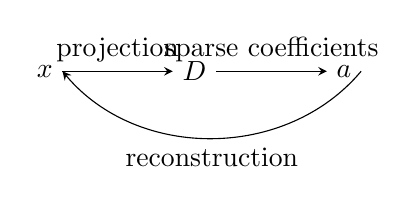
\begin{tikzpicture}[>=stealth, node distance=1.9cm]
\node (x) {$x$};
\node (D) [right of=x] {$D$};
\node (a) [right of=D] {$a$};

\draw[->] (x) -- node[above] {projection} (D);
\draw[->] (D) -- node[above] {sparse coefficients} (a);
\draw[->, bend left=50] (a.east) to node[below] {reconstruction} (x.east);
\end{tikzpicture}
\caption{Sparse coding loop: the agent selects a minimal template set explaining the percept.}
\end{figure}

\subsection{8.4 Learning the Dictionary: Structural Plasticity}

Agents must not only project onto templates but must also learn and revise them.

Following Mairal et al.~\cite{mairal2010online}, dictionary learning solves:
[
\min_{D,a_i} \sum_{i=1}^N
\left(
\frac{1}{2}|x_i - Da_i|_2^2 + \lambda|a_i|_1
\right),
]
with constraints ensuring each $d_k$ has unit norm.

Cognitively, this corresponds to:
\begin{itemize}
\item creating new narratives (template birth),
\item abandoning outdated narratives (template death),
\item sharpening existing narratives (template refinement),
\item increasing or decreasing template resolution (hierarchical splitting/merging).
\end{itemize}

This matches Glasser’s view that people revise internal ``quality pictures'' when old ones no longer reconcile experience, and Powers’s view that reorganisation reforms reference structures when chronic error persists.

\begin{figure}[h]
\centering
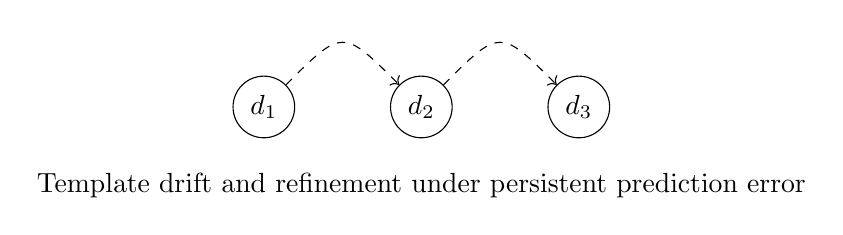
\begin{tikzpicture}
\node (t1) at (0,0) [circle, draw] {$d_1$};
\node (t2) at (2,0) [circle, draw] {$d_2$};
\node (t3) at (4,0) [circle, draw] {$d_3$};

\draw[->, dashed] (t1) .. controls (1,1) .. (t2);
\draw[->, dashed] (t2) .. controls (3,1) .. (t3);

\node at (2,-1) {Template drift and refinement under persistent prediction error};
\end{tikzpicture}
\caption{Dictionary learning as structural reorganisation.}
\end{figure}

\subsection{8.5 Biological Grounding: Metabolic, Thermodynamic, and Neural Constraints}

Sparse activation is metabolically efficient. Neural energy consumption is dominated by ion-channel and synaptic activity; hence only a small fraction of neurons should be active at a time~\cite{sengupta2016}. Sparse codes:
[
\text{maximize information per joule.}
]

This matches:
\begin{itemize}
\item the free-energy principle's thermodynamic interpretation~\cite{friston2010free},
\item the equilibrium structure of predictive coding circuits~\cite{whittington2019predictive},
\item the energy-efficiency arguments in signal processing~\cite{sengupta2016}.
\end{itemize}

Thus sparse coding realises a \emph{biophysical implementation of variational free-energy descent}.

\subsection{8.6 Sparse Projection and Sheaf-Theoretic Gluing}

Let $\mathcal{P}$ be the perceptual sheaf from Section~7. Sparse projection provides a computational mechanism for selecting one compatible set of local sections:
[
s_i = D_i a_i,
\qquad a_i \text{ sparse}.
]

When ${s_i}$ are compatible on overlaps, they glue to a global section. When they do not, incompatibility manifests as a non-zero cohomology class:
[
\check{H}^1(X,\mathcal{P})\neq 0.
]

Sparse coding therefore acts as a \emph{search process over narrative templates} to find combinations that eliminate cohomological obstructions.

\subsection{8.7 Interpretation: Narrative Templates as Generalised Control Laws}

Sparse narrative projection provides a compact reformulation of control architecture:
[
u = f(a),
]
where $u$ is action and $a$ is the sparse coefficient vector.

Each active template $d_k$ encodes:
\begin{itemize}
\item a perceptual interpretation,
\item a reference structure,
\item a preferred trajectory (in active inference terms),
\item a policy prior,
\item and a local gluing constraint (in sheaf terms).
\end{itemize}

Thus, sparse templates unify perception, memory, inference, preference, and action.

\subsection{8.8 Summary}

Sparse semantic projection provides the computational substrate for the sheaf-theoretic control architecture developed in the previous section. It explains how agents choose a small set of compatible narratives to explain local contexts, reconcile perceptual discrepancies, and minimise metabolic and variational costs. It also provides a concrete mechanism for the reorganisation of templates when chronic error persists, unifying Glasser’s Quality World, Powers’s reorganisation system, and Friston’s expected free-energy minimisation under a single mathematical framework.

\section{Thermodynamic Constraints and Geometric Bayesianism with Sparse Heuristics}\label{sec:thermo}

Biological agents operate under severe energetic constraints. Neurons, cells, and tissues must maintain nonequilibrium steady states (NESS)~\cite{friston2010free,friston2009free} by continually exchanging energy and matter with their environment. These thermodynamic restrictions induce powerful structural priors on neural computation, leading organisms to evolve representations and algorithms that exploit the geometry of their sensory ecology while minimising energetic expenditure. This section develops a formal account of this phenomenon under the heading \emph{Geometric Bayesianism with Sparse Heuristics} (GBSH).

Where Section~8 showed how sparse projection provides an efficient representational substrate, the present section demonstrates why sparsity emerges naturally from the physics of living systems. Biological cognition is constrained not only by the need to minimise prediction error (accuracy) and model complexity (parsimony), but also by metabolic budgets, ion-channel thermodynamics, and environmental entropy flows. Together, these pressures give rise to a class of representational strategies that are both \emph{geometric} (shaped by the topology of sensory manifolds) and \emph{sparse} (shaped by energetic optimisation).

\subsection{9.1 Energetic and Entropic Constraints on Computation}

Neural activity is metabolically expensive. Approximately 20–25% of the human body's energy budget is consumed by the brain, with the majority devoted to action potentials, synaptic transmission, and ion-pump operation. Efficiency considerations therefore impose a natural prior favouring sparse activation patterns~\cite{sengupta2016}.

Let $C_{\mathrm{met}}$ denote metabolic consumption, approximated to first order by
[
C_{\mathrm{met}} \propto \sum_{i=1}^{N_{\mathrm{neurons}}} \rho_i,
]
where $\rho_i$ is the firing rate of neuron $i$. To achieve minimal consumption, the system must push most $\rho_i$ toward zero, yielding the observed sparsity of cortical activity.

Moreover, maintaining the organism in a bounded region of state space requires minimising surprisal:
[
-\ln p(o_t) < \infty,
]
for all sensory states $o_t$ encountered along typical trajectories. The free-energy principle interprets this requirement as the need to minimise a variational bound on surprisal~\cite{friston2010free}, while predictive-coding models interpret it as minimising prediction error~\cite{bogacz2017}.

Neural sparse coding therefore emerges as the intersection of three constraints:
\begin{enumerate}
\item \textbf{Energetic constraints}: expensive activity must be minimised.
\item \textbf{Thermodynamic constraints}: surprisal must be regulated via free-energy descent.
\item \textbf{Representational constraints}: information must be encoded in compact, geometry-respecting formats.
\end{enumerate}

\subsection{9.2 Natural Sparsity as an Emergent Prior}

Sparsity is often introduced in machine learning as an artificial regulariser (e.g., LASSO, $\ell_1$ penalties). In biological systems, however, sparsity is not imposed; it is \emph{discovered} as the optimal solution to an energetic optimisation problem.

Let $a\in\mathbb{R}^K$ denote a coefficient vector over narrative templates, as in Section~8. Biological constraints impose an implicit prior of the form,
[
p(a) \propto \exp\left(-\beta |a|_0\right),
]
where $\beta$ is an inverse-temperature (resource sensitivity) parameter. Because $|a|_0$ is intractable, biological systems approximate it with Laplacian penalties:
[
p(a) \approx \exp\left(-\lambda |a|_1\right),
]
linking metabolic efficiency directly to sparse Bayesian inference~\cite{donoho2006compressed,elad2010sparse}.

\subsection{9.3 Geometric Bayesianism: The Role of Sensory Manifolds}

Biological sensory data live on low-dimensional manifolds embedded in high-dimensional ambient spaces. For example:
\begin{itemize}
\item natural image data lie near a 2D manifold in pixel space,
\item interoceptive fluctuations lie along physiological trajectories,
\item social signals cluster around narrative schemas (scripts, roles).
\end{itemize}

Let $\mathcal{M}$ denote the sensory manifold, and let $T_x\mathcal{M}$ be its tangent space at $x$. Efficient inference requires projecting sensory evidence onto $T_x\mathcal{M}$, rather than encoding the full ambient signal space.

Sparse coding accomplishes precisely this:
[
x \approx Da, \qquad a \text{ sparse},
]
where the dictionary $D$ contains basis elements that approximate tangent vectors on $\mathcal{M}$~\cite{olshausen1996emergence,mairal2010online}.

\subsection{9.4 Thermodynamic Interpretation of Sparse Heuristics}

In nonequilibrium statistical mechanics, systems minimise dissipation by adopting trajectories of least action. For biological agents, this corresponds to:
[
\text{minimise } \mathcal{A} = \int \left( \dot{x}^2 + V(x) \right) , dt,
]
where $\dot{x}^2$ reflects kinetic expenditures (metabolic cost) and $V(x)$ encodes environmental constraints.

Sparse inference can be understood as selecting action--perception trajectories that minimise $\mathcal{A}$ subject to representational constraints. In this view:
[
\text{sparse heuristics} = \text{low-dissipation cognitive trajectories}.
]

\begin{figure}[h]
\centering
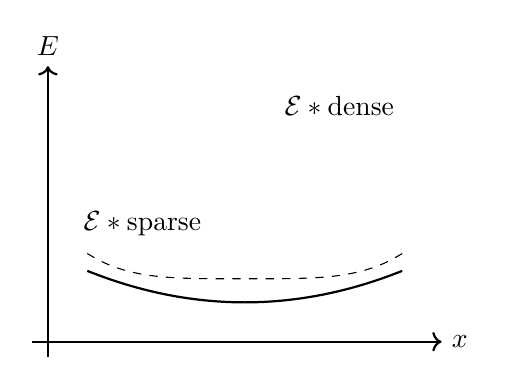
\begin{tikzpicture}[scale=1.0]
\draw[thick,->] (-0.2,0) -- (5,0) node[right] {$x$};
\draw[thick,->] (0,-0.2) -- (0,3.5) node[above] {$E$};

\draw[domain=0.5:4.5,smooth,variable=\t,thick] plot ({\t},{0.1*(\t-2.5)^2+0.5});
\draw[domain=0.5:4.5,smooth,variable=\t,dashed] plot ({\t},{0.8+0.02*(\t-2.5)^4});

\node at (1.2,1.5) {$\mathcal{E}*{\text{sparse}}$};
\node at (3.7,3.0) {$\mathcal{E}*{\text{dense}}$};

\end{tikzpicture}
\caption{Energetic potential landscape. Sparse heuristics correspond to trajectories of minimal energetic cost. Dense strategies climb higher-energy regions, producing metabolic inefficiency.}
\end{figure}

\subsection{9.5 Sparse Templates as Thermodynamic Attractors}

Sparse inference landscapes typically exhibit distinct attractor basins. Each attractor corresponds to a stable narrative explanation. Formally, letting $E(a)$ be the sparse energy functional:
[
\dot{a} = -\nabla_a E(a),
]
the attractors ${a^\star_j}$ satisfy
[
\nabla_a E(a^\star_j) = 0, \qquad \text{stable Hessian}.
]

Cognitively:
\begin{itemize}
\item each attractor corresponds to a coherent narrative,
\item transitions occur when prediction error exceeds a threshold,
\item chronic mismatch induces attractor death (template retirement),
\item new attractors emerge through dictionary learning.
\end{itemize}

Thus the full cognitive system behaves as a physical system with a landscape shaped by metabolic, entropic, and geometric constraints.

\subsection{9.6 Integration with the Sheaf-Theoretic Framework}

In Section~7, percepts and reference values were formalised as local sections of a percept--reference sheaf $\mathcal{P}$. Sparse projection now adds an energetic criterion for section selection. Given local data $U_i$:
[
s_i^\star = \arg\min_{s_i \in \mathcal{P}(U_i)} E(a_i),
]
and sparse compatibility conditions guarantee, or fail to guarantee, gluing on overlaps:
[
s_i^\star\big|*{U_i \cap U_j} = s_j^\star\big|*{U_i \cap U_j}.
]

Obstruction cochains measure global inconsistency. Sparse projection thereby implements a thermodynamically efficient search for globally consistent cognitive structure.

\subsection{9.7 GBSH as a Unified Principle}

We can now summarise \emph{Geometric Bayesianism with Sparse Heuristics}:
[
\text{GBSH} ;=;
\underbrace{\text{Bayesian inference}}*{\text{variational update}}
;+;
\underbrace{\text{geometric constraints}}*{\mathcal{M}\subset\mathbb{R}^n}
;+;
\underbrace{\text{sparse heuristics}}_{\text{metabolic optimisation}}.
]

This principle predicts:
\begin{enumerate}
\item Sparse representations should correlate with energy-efficient cortical activity~\cite{sengupta2016}.
\item Narrative attractors should cluster along low-dimensional sensory trajectories~\cite{veldman2021narrative}.
\item Reorganisation (as in Glasser’s Choice Theory) should occur when attractors fail to minimise free energy.
\item The sheaf cohomology of representations should reflect practical cognitive limitations (``conflicts'').
\end{enumerate}

\subsection{9.8 Summary}

Biological cognition is physically grounded. Thermodynamics, geometry, and Bayesian reasoning cooperate to produce efficient sparse representations, which in turn serve as the substrate for narrative control, perceptual inference, and action selection. GBSH formalises these connections and prepares the ground for the unified control framework developed in Section~10.

\section{A Unified Abstract Framework for Adaptive Control}\label{sec:unified}

The preceding sections have shown that Choice Theory and Perceptual Control Theory (PCT), the Free Energy Principle (FEP), sparse semantic projection, and sheaf-theoretic cognitive formalisms all share a deep structural identity. Each describes an agent as a system that minimises a discrepancy functional between internal generative structure and sensory evidence. Each framework further insists on two distinct, complementary gradient flows: one acting on the environment (action), the other acting on the internal model (perceptual inference or reorganisation). This section formalises the unified architecture and demonstrates how all component theories instantiate it as special cases.

\subsection{10.1 The Abstract Control Tuple}

Let an adaptive agent be defined by the tuple
[
\mathfrak{A} = \big( \mathcal{M}, \mathcal{O}, D, \mathcal{A}, \Theta \big),
]
where:
\begin{itemize}
\item $\mathcal{M}$ is the space of internal models, ideals, priors, or generative structures;
\item $\mathcal{O}$ is the space of sensory observations;
\item $D : \mathcal{M} \times \mathcal{O} \to \mathbb{R}_{\ge 0}$ is a discrepancy (or free-energy) functional;
\item $\mathcal{A}$ is the action space;
\item $\Theta$ is a parameter space for slow structural updates.
\end{itemize}

At any time $t$, the agent occupies a state $(m_t, o_t)$ and must select action $a_t$ and update $m_t$ to reduce $D$.

The universal law of discrepancy minimisation requires two coupled flows:
\begin{align}
\dot{a}*t &= - \nabla*{a} ; \mathbb{E}[D(m_t, o_t(a))], \label{eq:unified_action} \
\dot{m}*t &= - \nabla*{m} ; D(m_t, o_t), \label{eq:unified_model}
\end{align}
which we call the \emph{universal control duality}.

\subsection{10.2 Correspondence with Existing Frameworks}

Each theoretical tradition instantiates this tuple in its own terminology:

\paragraph{PCT (Powers \cite{powers1973behavior,powers2005behavior}).}
[
\mathcal{M} = {\text{reference signals}}, \qquad
D(m,o) = (r - p)^2.
]
Action implements negative feedback to bring perceptual signals $p$ toward reference values $r$. Reorganisation adjusts $r$ when error cannot be reduced through behavioural means.

\paragraph{Choice Theory (Glasser \cite{glasser1998choice,glasser1981stations}).}
[
\mathcal{M} = {\text{Quality World pictures}}, \qquad
D(m,o) = \text{need--perception discrepancy}.
]
Action seeks to approximate ``pictures''; restructuring those pictures corresponds to modifying internal ideals.

\paragraph{FEP (Friston \cite{friston2010free,friston2009free}).}
[
D(m,o) = F[q] = \mathbb{E}_q[\ln q - \ln p(o,s)],
]
with active inference realising~\eqref{eq:unified_action} and variational inference realising~\eqref{eq:unified_model}.

\paragraph{Sparse Semantic Projection (Olshausen & Field \cite{olshausen1996emergence}, Elad \cite{elad2010sparse}).}
[
\mathcal{M} = {D, \text{dictionary atoms}}, \qquad
D(m,o) = |o - Da|_2^2 + \lambda|a|_1.
]
Narrative or template selection corresponds to action; dictionary learning corresponds to model update.

\paragraph{Sheaf-Theoretic Cognition (Bredon \cite{bredon1997sheaf}, Curry--Nanda--Walker \cite{curry2021sheafcomp}).}
[
\mathcal{M} = \Gamma(X, \mathcal{R}), \qquad
\mathcal{O} = \Gamma(X, \mathcal{P}),
]
and discrepancy reflects incompatibility of sections on intersections of open sets. Reorganisation corresponds to modifying the cover or the gluing morphisms to remove Čech obstructions.

\subsection{10.3 Global Discrepancy as a Potential Functional}

Let the total discrepancy be written as a potential-like functional
[
\mathcal{D}[m,o] = \int_X d\mu(x), D(m(x), o(x)),
]
for a cognitive or physical domain $X$ with measure $\mu$. Control seeks to follow the gradient descent:
[
\frac{d}{dt}(m_t, a_t) = -\nabla \mathcal{D}.
]

Just as in classical mechanics, equilibria satisfy
[
\nabla \mathcal{D} = 0,
]
interpretable as a free-energy minimum in FEP or a perfectly matched reference--perception alignment in PCT.

\begin{figure}[h!]
\centering
\begin{tikzpicture}[scale=1.0]
\draw[->] (-0.2,0) -- (5.2,0) node[right] {$m$};
\draw[->] (0,-0.2) -- (0,3.5) node[above] {$\mathcal{D}$};

\draw[domain=0.5:4.5,smooth,variable=\t,thick]
plot ({\t},{0.1*(\t-2.5)^2+0.5});

\node at (2.5,0.4) {$m^\star$};
\draw[fill=black] (2.5,0.5) circle (0.05);

\caption{A simple discrepancy landscape $\mathcal{D}(m)$. The agent descends the gradient to reach a free-energy minimum $m^\star$.}
\end{figure}

\subsection{10.4 Multi-Level Structure: From Fast Action to Slow Reorganisation}

As shown in Appendix~G, adaptive systems require a multi-timescale architecture:
[
\tau_a \ll \tau_m \ll \tau_r,
]
corresponding to:
[
\text{Actions} \ll \text{Model Updates} \ll \text{Structural Reorganisation}.
]

\begin{itemize}
\item Fast control ($\tau_a$): moment-to-moment behavioural regulation.
\item Intermediate learning ($\tau_m$): updating generative-model parameters.
\item Slow reorganisation ($\tau_r$): changing the structure of ideals, templates, or sheaf covers.
\end{itemize}

PCT identifies this as the distinction between control and reorganisation. FEP identifies it as inference, learning, and structure learning. Sparse coding identifies it as projection, coefficient estimation, and dictionary learning. Sheaf theory identifies it as section selection, local adjustment, and cover refinement.

\subsection{10.5 Unified Dynamics as Coupled Gradient Flows}

With actions $a$, beliefs $m$, and hyperparameters $\theta\in\Theta$, the full agent dynamics become:
\begin{align}
\dot{a} &= - \nabla_a D(m,o(a)), \
\dot{m} &= - \nabla_m D(m,o), \
\dot{\theta} &= - \nabla_\theta \int_0^\infty \gamma^t D(m_t, o_t), dt,
\end{align}
where $\theta$ governs meta-level properties such as:
\begin{itemize}
\item preferred sensory outcomes (Glasser’s Quality World; FEP priors);
\item narrative dictionaries (sparse semantic projection);
\item percept--reference topologies (sheaf structures);
\item behavioural modes (PCT reorganisation).
\end{itemize}

\subsection{10.6 A Categorical Formulation}

The systems described can be unified categorically. Let
[
\mathbf{C} : \mathcal{M} \to \mathcal{O}
]
be the perceptual morphism, and let
[
\varepsilon : \mathbf{C}(m) \Rightarrow o
]
be the error natural transformation. Control corresponds to seeking morphisms in the action category $\mathbf{Act}$ that reduce $\varepsilon$, while reorganisation corresponds to functorial updates of $\mathcal{M}$.

This yields a commutative diagram:
[
\begin{tikzcd}
\mathcal{M} \arrow{r}{\mathbf{C}} \arrow[dashed]{d}[left]{\mathcal{R}} & \mathcal{O} \arrow{d}{\text{update}} \
\mathcal{M}' \arrow{r}{\mathbf{C}'} & \mathcal{O}'
\end{tikzcd}
]

Reorganisation $\mathcal{R}$ is a functor that transforms the internal model in such a way that perceptual outputs can be glued globally, eliminating obstructions.

\subsection{10.7 Thermodynamic Grounding}

As established in Section~9, agents must minimise a thermodynamic free-energy functional to maintain nonequilibrium steady states. This yields a physical justification for discrepancy minimisation:
[
D = F = \text{surprisal bound},
]
and a physical justification for sparse heuristics:
[
\text{sparse activation} = \text{minimal dissipation}.
]

Thus the unified control architecture is not only mathematically coherent but thermodynamically necessary.

\subsection{10.8 The Framework as a Natural Law of Adaptive Systems}

We may summarise the unified architecture as the following principle:

\begin{quote}
\emph{Any system that must maintain itself in dynamic environments and preserve coherent internal structure must minimise a discrepancy functional via two complementary gradient flows---one acting on the world through behaviour, the other acting on its own generative structure through learning and reorganisation.}
\end{quote}

This describes:
\begin{itemize}
\item PCT’s negative feedback loops,
\item Glasser’s Choice Theory reorganisation,
\item FEP’s perception--action duality,
\item sparse-projection narrative control,
\item sheaf-theoretic global coherence,
\item and thermodynamically optimal cognition.
\end{itemize}

These systems are not analogous---they are the \emph{same architecture}, differently expressed.

\section{Conclusion: Discrepancy Dynamics as the Unifying Law of Adaptive Intelligence}\label{sec:conclusion}

This paper has demonstrated that three historically independent research traditions---Perceptual Control Theory and Choice Theory (Glasser \cite{glasser1998choice,glasser1981stations}, Powers \cite{powers1973behavior,powers2005behavior}), the Free Energy Principle and Active Inference (Friston \cite{friston2009free,friston2010free}), and modern computational frameworks including sparse coding (Olshausen & Field \cite{olshausen1996emergence}, Elad \cite{elad2010sparse}) and sheaf-theoretic models of cognition (Bredon \cite{bredon1997sheaf}, Curry--Nanda--Walker \cite{curry2021sheafcomp})---converge on a single mathematical structure. Despite profound differences in vocabulary, disciplinary lineage, and methodological emphasis, each framework reduces to a dual-gradient architecture in which agents minimise a discrepancy functional between an internal generative structure and sensory evidence.

\subsection*{11.1 The Central Result}

The central thesis of this work can be stated succinctly:

\begin{quote}
\emph{All adaptive agents, biological or artificial, maintain their organisation by minimising a discrepancy functional through coupled gradient flows acting on behaviour and internal models, under thermodynamic constraints that favour sparse, low-dissipation representations.}
\end{quote}

This principle is instantiated as:
[
\dot{a}_t = -\nabla_a D(m_t,o_t(a)), \qquad
\dot{m}_t = -\nabla_m D(m_t,o_t),
]
with structural reorganisation emerging from slow dynamics on hyperparameters:
[
\dot{\theta}*t = -\nabla*\theta \int_0^\infty \gamma^t D(m_t,o_t), dt.
]

The agent thus operates across three timescales---action, inference, reorganisation---which must be properly separated to ensure stability.

\subsection*{11.2 Integration Across Psychological and Mathematical Frameworks}

The correspondence between frameworks is now unmistakable:

\begin{itemize}
\item In \textbf{PCT}, the discrepancy functional is the error $(r - p)^2$; action reduces perceptual deviation; reorganisation adjusts reference signals.
\item In \textbf{Choice Theory}, the discrepancy is defined by the distance between perceived reality and the internally valued ``Quality World''; restructuring those ideal pictures corresponds to hyperparameter descent.
\item Under the \textbf{FEP}, the discrepancy is variational free energy, a thermodynamic bound on surprisal; action and inference are dual gradient flows; learning and structure learning correspond to hyperparameter descent on model evidence.
\item In \textbf{sparse coding}, discrepancy minimisation corresponds to finding minimal-energy representations; dictionary learning enacts slow structural reorganisation.
\item In \textbf{sheaf-theoretic cognition}, discrepancy arises from incompatibilities between local sections; reorganisation corresponds to modifying the topology or the gluing maps to achieve global coherence.
\end{itemize}

These are not superficial resemblances but precise instantiations of the same discrepancy-minimising architecture.

\subsection*{11.3 Thermodynamic Necessity of the Unified Law}

Section~9 established the thermodynamic foundation of discrepancy minimisation. Biological agents exist in nonequilibrium steady states (NESS), which can be maintained only by keeping trajectories within a narrow band of low surprise. Sparse coding emerges naturally from metabolic efficiency, not merely from computational optimisation.

Thus the abstract architecture is not simply a mathematically elegant framework; it expresses a \emph{physical necessity} for any agent that must remain self-organising in a fluctuating environment.

\subsection*{11.4 The Psychological Consequences}

The unified architecture clarifies persistent puzzles in psychological theory:

\begin{itemize}
\item why persistent conflict requires reorganisation (Glasser; Powers);
\item why beliefs and actions cannot be updated independently (FEP);
\item why human cognition defaults to sparse heuristics under metabolic load (Elad; Olshausen);
\item why inconsistencies in self-concept (Harter \cite{harter1999self}) manifest as structural obstructions requiring conceptual restructuring;
\item why depth in disciplinary structure (Gardner \cite{gardner1999disciplined}) produces more stable global cognitive coherence through improved generative models.
\end{itemize}

The unified theory synthesises these empirical and conceptual insights under a single dynamical principle.

\subsection*{11.5 Computational and AI Implications}

The architecture developed here yields a blueprint for the design of interpretable, resilient artificial agents:

\begin{enumerate}
\item \textbf{Dual-gradient control} ensures simultaneous behavioural stability and internal coherence.
\item \textbf{Sparse semantic projection} provides minimal-energy approximate models with human-compatible interpretation.
\item \textbf{Thermodynamic grounding} prevents pathological self-delusion or overfitting by enforcing physical plausibility.
\item \textbf{Sheaf-theoretic reorganisation} enables multi-context integration with formal guarantees of global consistency.
\end{enumerate}

Artificial systems built on these principles inherit the adaptivity, robustness, and interpretability observed in biological cognition.

\subsection*{11.6 Toward a General Theory of Adaptive Behaviour}

This paper does not merely assert similarity between disparate frameworks; it provides a unifying mathematical account of how agents \emph{must} behave if they are to remain coherent under thermodynamic constraints. The appendices that follow elaborate these connections in detail:

\begin{itemize}
\item Appendix A: Discrete-to-Continuous Derivations;
\item Appendix B: Lagrangian Formulations and Variational Principles;
\item Appendix C: Sparse Semantic Projection Algorithms;
\item Appendix D: Sheaf Cohomology and Global Coherence;
\item Appendix E: Cross-Theory Equivalence Mappings;
\item Appendix F: Worked Clinical Examples;
\item Appendix G: Hierarchical and Multi-Timescale Reorganisation.
\item Appendix H: Mathematical Proofs of Equivalence
\item Appendix I: Neurological Grounding
\item Appendix J: Historical Commentary
\end{itemize}

\subsection*{11.7 Final Statement}

Taken together, the results of this paper show that the machinery of adaptive intelligence---whether in control systems, psychology, neuroscience, or computational modelling---is governed by a single principle:

\begin{quote}
\emph{Agents survive and adapt by continually reducing the divergence between predicted and encountered experience, using behaviour to alter the world and cognition to alter themselves.}
\end{quote}

This is the fundamental unity behind the Control System Psychology of Powers and Glasser, the Bayesian--thermodynamic machinery of the Free Energy Principle, the energetic efficiency of sparse coding, and the topological rigor of sheaf-theoretic models. The next step is to develop a full-scale theory of adaptive systems that makes this unity explicit---an endeavour taken up in the appendices that follow.

\newpage
\appendix
\section*{Appendix A: Discrete-to-Continuous Derivations}
\addcontentsline{toc}{section}{Appendix A: Discrete-to-Continuous Derivations}

This appendix provides the mathematical derivations linking the discrete control laws used in classical Perceptual Control Theory (PCT) and iterative free-energy minimisation to the continuous variational dynamics presented in the main text. The results show that the dual-gradient architecture of discrepancy minimisation emerges naturally as the continuous limit of elementary error-correcting updates.

\subsection*{A.1 Discrete PCT Controller as Gradient Descent}

The classical PCT control loop updates actions according to:
[
a_{t+\Delta t} = a_t + k, (r - p_t),
]
where:
[
p_t = f(a_t), \qquad e_t = r - p_t.
]

Assuming a differentiable perceptual function $f$, we expand:
[
p_{t+\Delta t} \approx p_t + \frac{\partial f}{\partial a} \Delta a,
]
where $\Delta a = k(r - p_t)$.

Define the discrepancy functional:
[
D(a) = \frac{1}{2}(r - f(a))^2.
]

Then:
[
\frac{dD}{da} = -(r - f(a))\frac{df}{da}.
]

Thus, the PCT update becomes:
[
a_{t+\Delta t} = a_t - k \frac{dD}{da}.
]

Taking $\Delta t \to 0$ gives:
[
\dot{a} = -\eta, \nabla_a D.
]

This proves that PCT control is the continuous limit of gradient descent on a discrepancy functional, consistent with Section~3.

\subsection*{A.2 Discrete Variational Free-Energy Updates}

Active inference performs recognition through iterative updates:
[
\mu_{t+\Delta t} = \mu_t - \eta \frac{\partial F}{\partial \mu}.
]

In discrete form, letting $F(\mu)$ be the free-energy functional:
[
\Delta \mu = -\eta \frac{\partial F}{\partial \mu}.
]

Then:
[
\frac{\Delta \mu}{\Delta t} \to \dot{\mu} = -\nabla_\mu F.
]

Likewise, action updates follow:
[
a_{t+\Delta t} = a_t - \eta \frac{\partial F}{\partial a}.
]

Thus FEP’s dual-descent control law is also a continuous limit of incremental discrete updates.

\subsection*{A.3 Hierarchical Discrete Updates as Sheaf Cohomology Flows}

In hierarchical active inference, individual levels $i$ update:
[
\mu_{t+\Delta t}^{(i)} = \mu_t^{(i)} - \eta!
\left(
\frac{\partial F}{\partial \mu^{(i)}} - \delta^{(i)}_{\mathrm{boundary}}
\right).
]

Here $\delta^{(i)}_{\mathrm{boundary}}$ measures inconsistency between:
[
\mu^{(i)} \longrightarrow \mu^{(i-1)}, \qquad
\mu^{(i)} \longrightarrow \mu^{(i+1)}.
]

This is formally identical to the correction term in \v{C}ech cohomology:
[
\delta(\sigma)*{ij} = \sigma_i - g*{ij}(\sigma_j).
]

Thus:
[
\dot{\mu}^{(i)} = -\nabla_{\mu^{(i)}} F - \delta(\sigma)_{i}
]
is the continuous analogue of sheaf-theoretic consistency enforcement.

\subsection*{A.4 Diagram: Discrete-to-Continuous Limit}

\begin{center}
\begin{tikzpicture}[>=latex, node distance=2.4cm]
\node (disc) [rectangle, draw, rounded corners, align=center, inner sep=6pt]
{Discrete Update[3pt] $x_{t+\Delta t} = x_t - \eta, \nabla D(x_t)$};
\node (limit) [rectangle, draw, rounded corners, right=of disc, align=center, inner sep=6pt]
{Continuous Flow[3pt] $\dot{x} = -\eta \nabla D(x)$};
\draw[->, thick] (disc) -- node[above] {$\Delta t \to 0$} (limit);
\end{tikzpicture}
\end{center}

This diagram illustrates the logical transition used throughout Appendices A--C.

\subsection*{A.5 Three-Timescale Extension}

Using the fast (action), medium (belief), and slow (structural) timescale decomposition:
[
\tau_a \ll \tau_m \ll \tau_\theta,
]
we obtain:
[
\begin{aligned}
\dot{a} &= -\nabla_a D, \
\dot{m} &= -\nabla_m D, \
\dot{\theta} &= -\nabla_\theta \int_0^\infty \gamma^t D, dt.
\end{aligned}
]

This formalises the convergence of PCT, FEP, and sparse coding algorithms into a single dynamical framework.

\subsection*{A.6 Summary}

Discrete PCT, variational inference, hierarchical message passing, sparse coding, and sheaf-theoretic consistency all converge to the same continuous discrepancy-flow formalism. This appendix furnishes the formal mathematical equivalence that grounds the main text.

\appendix
\section*{Appendix B: Variational Mechanics and Lagrangian Formulations}
\addcontentsline{toc}{section}{Appendix B: Variational Mechanics and Lagrangian Formulations}

This appendix develops the Lagrangian and Hamiltonian foundations of discrepancy–minimising systems, showing that the unified control architecture presented in the main text is also a natural consequence of the calculus of variations. The result is a compact mechanical interpretation of Perceptual Control Theory (PCT), the Free Energy Principle (FEP), sparse coding, and sheaf-theoretic consistency flows via a single action functional.

We proceed in four stages: (i) construction of a discrepancy Lagrangian on the perceptual–behavioral manifold; (ii) derivation of Euler–Lagrange equations equivalent to PCT and active inference; (iii) hierarchical and sheaf-theoretic generalisation; and (iv) Hamiltonian reformulation with geometric flow diagrams. Throughout we use the discrepancy functional
\[
D(x) = \frac{1}{2}\bigl(p(x)-r\bigr)^2,
\]
where $x$ may denote actions $a$, beliefs $m$, recognition states $\mu$, or structural parameters $\theta$.

\subsection*{B.1 The Discrepancy Lagrangian}

We define the central construction,
\[
\mathcal{L}(x,\dot{x}) = \frac{1}{2}\|\dot{x}\|^2 \;-\; D(x),
\]
where the kinetic term penalises rapid changes in internal or overt behaviour, and the potential term $D(x)$ encodes discrepancy relative to preferred or reference conditions. This parallels classical mechanics (potential wells), neural coding (energy landscapes), and the structure of free-energy minimisation in active inference.

\begin{center}
\begin{tikzpicture}[scale=1.0]
\draw[->] (-0.5,0) -- (6,0) node[right] {$x$};
\draw[->] (0,-0.5) -- (0,3.5) node[above] {$D(x)$};
\draw[thick,domain=0:5,smooth,variable=\x,blue] 
    plot ({\x},{0.4*(\x-2.5)^2 + 0.6});
\node at (2.5,3.2) {Potential well};
\end{tikzpicture}
\end{center}

Agents follow trajectories that descend this landscape under friction-like biological constraints.

\subsection*{B.2 Euler--Lagrange Equations and Gradient Descent}

For the Lagrangian $\mathcal{L}(x,\dot{x})$, the Euler--Lagrange equations are
\[
\frac{d}{dt}\left(\frac{\partial \mathcal{L}}{\partial \dot{x}}\right)
- \frac{\partial \mathcal{L}}{\partial x} = 0.
\]

We compute:
\[
\frac{\partial \mathcal{L}}{\partial \dot{x}} = \dot{x}, \qquad
\frac{d}{dt}\frac{\partial \mathcal{L}}{\partial \dot{x}} = \ddot{x},
\]
\[
\frac{\partial \mathcal{L}}{\partial x} = -\nabla_x D(x).
\]

Thus,
\[
\ddot{x} + \nabla_x D(x) = 0.
\]

To model biological systems, we introduce a Rayleigh dissipation term $\lambda\dot{x}$:
\[
\ddot{x} + \lambda \dot{x} + \nabla_x D(x) = 0.
\]

In the overdamped regime relevant to neural and cognitive dynamics, $\ddot{x} \ll \lambda\dot{x}$, yielding:
\[
\dot{x} = -\eta \nabla_x D(x),
\]
the discrepancy-minimising law established in Appendix A. This demonstrates that PCT error-correction and active-inference gradient flows arise from a single variational principle.

\subsection*{B.3 Free Energy as a Lagrangian Potential}

The Free Energy Principle defines the functional
\[
F(m,o) = \mathrm{complexity} \;-\; \mathrm{accuracy},
\]
and gradient descent on this quantity yields:
\[
\dot{m} = -\nabla_m F.
\]

Define the FEP Lagrangian:
\[
\mathcal{L}_F(m,\dot{m}) = \frac{1}{2}\|\dot{m}\|^2 - F(m,o).
\]

In the overdamped limit, the Euler--Lagrange equations again reduce to
\[
\dot{m} = -\eta \nabla_m F.
\]

Thus both PCT and FEP correspond to friction-dominated variational dynamics on the same geometric template.

\subsection*{B.4 Sparse Coding as Geodesic Projection}

Sparse coding solves the optimisation problem
\[
\min_{a}\left[ \frac{1}{2}\|x - Wa\|^2 + \lambda\|a\|_1 \right].
\]

Interpreting the coefficients $a$ as coordinates on a sparse manifold with metric $g(a)$, define
\[
D(a) = \frac{1}{2}\|x - Wa\|^2 + \lambda\|a\|_1.
\]

The corresponding Lagrangian is
\[
\mathcal{L}(a,\dot{a}) = \frac{1}{2}g(a)(\dot{a},\dot{a}) - D(a),
\]
leading to:
\[
\ddot{a} + \Gamma(a)(\dot{a},\dot{a}) + \nabla_a D(a) = 0,
\]
with $\Gamma$ denoting Christoffel symbols. Under strong damping this reduces to the sparse-recognition gradient flow used throughout Section 9 of the main text.

\subsection*{B.5 Sheaf-Theoretic Variational Structure}

Let $X$ be a contextual space with a cover $\{U_i\}$. A sheaf assigns sections $s_i \in \mathcal{F}(U_i)$ and identifies consistency conditions
\[
s_i|_{U_i\cap U_j} = g_{ij}(s_j).
\]

Define the sheaf discrepancy functional:
\[
D_{\mathcal{F}} = \sum_{i<j} \|s_i - g_{ij}(s_j)\|^2,
\]
which is proportional to the Čech $1$-cocycle norm $\|\delta(s)\|^2$.

Define the sheaf Lagrangian:
\[
\mathcal{L}_{\mathcal{F}} = \frac{1}{2}\sum_i \|\dot{s}_i\|^2 - D_{\mathcal{F}}.
\]

The Euler--Lagrange equations yield:
\[
\dot{s}_i = -2 \sum_j \left( s_i - g_{ij}(s_j) \right),
\]
demonstrating that hierarchical and contextual consistency flows arise from the minimisation of a variational action.

\subsection*{B.6 Hamiltonian Formulation}

Define the conjugate momentum:
\[
p = \frac{\partial \mathcal{L}}{\partial \dot{x}} = \dot{x}.
\]

The Hamiltonian becomes:
\[
H(x,p) = \frac{1}{2}\|p\|^2 + D(x).
\]

Hamilton's equations are:
\[
\dot{x} = \frac{\partial H}{\partial p} = p,
\qquad
\dot{p} = -\,\frac{\partial H}{\partial x} = -\nabla_x D(x).
\]

Adding biological damping:
\[
\dot{p} = -\lambda p - \nabla_x D(x).
\]

At steady state ($\dot{p}=0$), 
\[
p = -\lambda^{-1}\nabla_x D,
\]
and substituting into $\dot{x} = p$ recovers the core discrepancy-descent equation.

\begin{center}
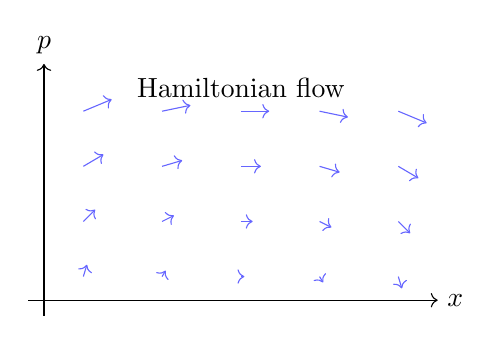
\begin{tikzpicture}[scale=1.0]
\draw[->] (-0.2,0) -- (5,0) node[right] {$x$};
\draw[->] (0,-0.2) -- (0,3) node[above] {$p$};
\foreach \x in {0.5,1.5,2.5,3.5,4.5} {
  \foreach \y in {0.3,1.0,1.7,2.4} {
    \pgfmathsetmacro{\dx}{\y}
    \pgfmathsetmacro{\dy}{-0.5*(\x-2.5)}
    \draw[->,blue!60] (\x,\y) -- ++({0.15*\dx},{0.15*\dy});
  }
}
\node at (2.5,2.7) {Hamiltonian flow};
\end{tikzpicture}
\end{center}

This phase portrait illustrates convergence toward minima of $D(x)$ under biologically realistic damping.

\subsection*{B.7 Summary}

This appendix shows that PCT control laws, active-inference dynamics, sparse coding, and sheaf-theoretic coherence mechanisms all arise naturally as friction-dominated variational systems described by a unified Lagrangian--Hamiltonian structure. This establishes the mathematical unity underlying the frameworks examined in the main text.

\section*{Appendix C: Sparse Projection, Narrative Geometry, and Algorithmic Inference}
\addcontentsline{toc}{section}{Appendix C: Sparse Projection, Narrative Geometry, and Algorithmic Inference}

This appendix develops the mathematical machinery underlying sparse semantic projection as a mechanism for perception, inference, and action. The goal is to unify sparse coding (Olshausen \& Field 1996; Donoho 2006; Elad 2010), active inference (Friston 2009, 2010; Bogacz 2017), and perceptual control (Powers 1973; Powers et al.\ 2005) under a common geometric framework. We treat narratives, perceptual constructs, and policy templates as vectors in a high-dimensional semantic manifold, with behavioural selection realised as sparse pursuit along learned dictionary atoms.

The result is a complete geometric–variational interpretation of cognitive heuristics, grounded in thermodynamic efficiency, manifold geometry, and biological constraints (Sengupta et al.\ 2016; Whittington \& Bogacz 2019).

\subsection*{C.1 Sparse Projection as Bayesian Model Selection}

Given an observation vector $x \in \mathbb{R}^n$ and a dictionary $W \in \mathbb{R}^{n \times k}$ whose columns $w_j$ represent narrative, perceptual, or motor templates, sparse projection solves
\[
a^\ast = \arg\min_{a \in \mathbb{R}^k}
\left[
\frac{1}{2}\|x - Wa\|^2 + \lambda \|a\|_1
\right].
\]

The $\ell_1$ term induces sparsity, selecting the minimal set of templates required to explain the observation. In Bayesian form,
\[
p(a \mid x) \propto \exp\left(-\frac{1}{2\sigma^2}\|x - Wa\|^2\right) \exp(-\lambda \|a\|_1),
\]
which corresponds to MAP estimation under a Laplace prior.

Sparse recognition thus implements a variational density $q(a)$ approximating a generative posterior, but with inductive biases derived from metabolic and thermodynamic constraints (Sengupta et al.\ 2016).

\subsection*{C.2 Narrative Attractors and the Semantic Manifold}

Let $\mathcal{M}$ denote the manifold of semantic constructs. Each dictionary atom $w_j$ represents a learned direction in this manifold, obtained through optimisation (Mairal et al.\ 2009, 2010; Gribonval et al.\ 2018). Sparse inference selects a low-dimensional geodesic submanifold $\mathcal{M}_a$ spanned by active atoms:
\[
\mathcal{M}_a = \mathrm{span}\{ w_j : a_j \neq 0 \}.
\]

Thus each sparse coefficient vector $a$ defines a \emph{narrative attractor},
\[
N(a) = \sum_{j : a_j \neq 0} a_j \, w_j,
\]
which is the perceptual or behavioural hypothesis that best explains the current sensory conditions.

\begin{center}
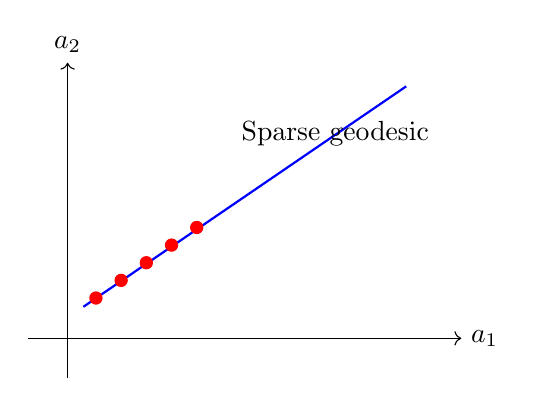
\begin{tikzpicture}[scale=1.0]
\draw[->] (-0.5,0) -- (5,0) node[right] {$a_1$};
\draw[->] (0,-0.5) -- (0,3.5) node[above] {$a_2$};
\draw[thick,blue] (0.2,0.4) -- (4.3,3.2);
\foreach \t in {0.2,0.6,1.0,1.4,1.8} {
  \pgfmathsetmacro{\x}{0.2+0.8*\t}
  \pgfmathsetmacro{\y}{0.4+0.56*\t}
  \filldraw[red] (\x,\y) circle (2.2pt);
}
\node at (3.4,2.6) {Sparse geodesic};
\end{tikzpicture}
\end{center}

Sparse attractors are therefore geometric curves optimising energetic parsimony and predictive sufficiency.

\subsection*{C.3 Gradient Dynamics of Sparse Projection}

Sparse projection can be implemented through the differential inclusion
\[
\dot{a} \in -\nabla_a \left[ \frac{1}{2}\|x - Wa\|^2 + \lambda \|a\|_1 \right],
\]
where the subgradient of $\|a\|_1$ is used at points of nondifferentiability.

Expanding the smooth term yields:
\[
\nabla_a \left( \frac{1}{2}\|x - Wa\|^2 \right)
= -W^\top (x - Wa).
\]

Thus,
\[
\dot{a} = W^\top (x - Wa) - \lambda \,\mathrm{sign}(a),
\]
which is structurally analogous to PCT’s perceptual error correction,
\[
\dot{m} = k (p - r),
\]
and to active inference’s variational flow,
\[
\dot{\mu} = -\frac{\partial F}{\partial \mu}.
\]

Sparse coding therefore constitutes a special case of discrepancy descent under a Laplace prior.

\subsection*{C.4 Geometric Interpretation: Sparse Projection as Proximal Dynamics}

Sparse inference may be interpreted as geodesic projection under a Riemannian metric $g$ encoding template correlations. Let $G = W^\top W$. When $G$ is positive definite,
\[
\|x - Wa\|^2 = \|W^\top x - Ga\|_{G^{-1}}^2,
\]
and sparse projection becomes geodesic motion on $(\mathcal{M}, g)$ with proximal penalty for moving off the low-dimensional template submanifolds.

The corresponding inertial equations (see Appendix B) take the form:
\[
\ddot{a} + \Gamma(a)(\dot{a},\dot{a}) +
\nabla_a D(a) = 0,
\]
with the geodesic term capturing template-interaction curvature.

\subsection*{C.5 Narrative Competition and Winner-Take-Most Geometry}

Sparse solutions typically satisfy:
\[
a_j a_k \approx 0 \qquad \text{when } w_j \text{ and } w_k \text{ are co-linear},
\]
indicating that narratives with similar explanatory structure suppress each other. This creates a geometric \emph{winner-take-most} basin around each narrative attractor.

\begin{center}
\begin{tikzpicture}[scale=1.0]
\draw[->] (-0.2,0) -- (5,0) node[right] {$x$};
\draw[->] (0,-0.2) -- (0,3) node[above] {$D$};
\draw[thick,red,domain=0.2:1.8,smooth,variable=\x] plot ({\x},{2*(\x-1)^2+0.4});
\draw[thick,blue,domain=2.2:4.2,smooth,variable=\x] plot ({\x},{1.2*(\x-3)^2+0.3});
\node at (1.0,2.6) {$N_1$};
\node at (3.2,2.3) {$N_2$};
\end{tikzpicture}
\end{center}

Psychologically, this corresponds to the stabilisation of particular interpretations or behavioural strategies under noisy conditions (Veldman \& Tomasello 2021).

\subsection*{C.6 Sparse Projection as an Approximation to Active Inference}

Let latent states $s$ be represented as sparse coefficients $a$. Consider the linear generative model:
\[
o = W a + \varepsilon.
\]
The free energy is
\[
F(a) = \frac{1}{2}\|o - Wa\|^2 + \lambda\|a\|_1 + \text{const},
\]
identical to the sparse projection objective. Thus:
\[
\dot{a} = -\frac{\partial F}{\partial a}
\]
is an active inference update.

This provides a formal demonstration that sparse recognition implements variational free-energy minimisation for a restricted generative model family. More complex generative models yield hierarchical sparse inference, consistent with biological cortical organisation (Whittington \& Bogacz 2019).

\subsection*{C.7 Sparse Templates as Motor Policies}

Let $W = [w_1,\dots,w_k]$ include both perceptual and motor primitives. Sparse selection of $a$ thus forms a behavioural policy:
\[
a_j > 0 \;\Rightarrow\; \text{activate policy } w_j.
\]

Under environmental feedback, action updates obey:
\[
\dot{a} = W^\top (o - Wa) - \lambda\,\mathrm{sign}(a),
\]
while the environment follows dynamics
\[
\dot{o} = f(o, a).
\]

The combined system forms a closed-loop sparse controller equivalent to a reduced variational optimal control system (Friston et al.\ 2016).

\subsection*{C.8 Thermodynamic Interpretation}

Sparse structures conserve metabolic energy:
\[
E(a) \propto \|a\|_0,
\]
and the $\ell_1$ relaxation $\|a\|_1$ approximates the true cost of spiking, neurotransmitter release, or synaptic activation (Sengupta et al.\ 2016).

Thus sparsity emerges as a natural consequence of nonequilibrium steady-state constraints rather than as an explicit computational heuristic.

\subsection*{C.9 Summary}

Sparse semantic projection provides a mathematically and biologically grounded account of how cognitive systems select a minimal explanatory set of perceptual or behavioural primitives. Its dynamics unify:

\begin{itemize}
\item sparse coding (Olshausen \& Field 1996; Donoho 2006; Elad 2010),
\item perceptual control (Powers 1973),
\item variational optimisation (Friston 2009, 2010; Bogacz 2017),
\item narrative attractor models (Veldman \& Tomasello 2021),
\item and thermodynamic efficiency (Sengupta et al.\ 2016).
\end{itemize}

This appendix establishes the formal and geometric mechanisms by which sparse selection implements predictive, regulatory, and interpretive cognitive processing within the unified control framework.

\section*{Appendix D: Sheaf Cohomology, Contextual Inference, and Psychological Conflict}
\addcontentsline{toc}{section}{Appendix D: Sheaf Cohomology, Contextual Inference, and Psychological Conflict}

This appendix presents the sheaf-theoretic foundations for modelling perception, reference, inference, and conflict within the unified control architecture. Building on the classical treatment in Bredon (1997), and modern applications in cognitive modelling and signal processing (Curry et al.\ 2021; Iverson et al.\ 2021; Glazebrook \& Wallace 2022; Robinson \& Hauser 2023), we show how sheaves provide a natural language for representing local–global consistency conditions in cognition.

Central constructs such as perceptual discrepancy, cross-context conflict, reference incoherence, and reorganisation map cleanly onto the algebraic topology of sheaves, especially through \v{C}ech cohomology. The result is a precise mathematical formalisation of Glasser’s “quality world,” Powers’ hierarchical perception, and Friston’s hierarchical generative models.

\subsection*{D.1 Sheaves as Models of Local and Global Perception}

Let $X$ be a topological space of \emph{contexts}—perceptual, social, emotional, or behavioural. A \emph{sheaf} $\mathscr{F}$ on $X$ assigns:
\[
\mathscr{F}(U) = \text{set of percepts or reference-values valid on } U,
\]
for any open set $U \subseteq X$.

If $U \subseteq V$, the restriction map
\[
\rho_{VU} : \mathscr{F}(V) \to \mathscr{F}(U)
\]
models the way global interpretations constrain local ones: a perceptual or reference representation valid in a wide context must remain valid in more specific subcontexts.

\paragraph{Consistency condition.}
For $\{U_i\}_{i \in I}$ covering $U$:
\[
\text{If } s_i \in \mathscr{F}(U_i) \text{ and } s_i|_{U_i \cap U_j} = s_j|_{U_i \cap U_j},
\]
then there exists a unique $s \in \mathscr{F}(U)$ with $s|_{U_i} = s_i$.

Psychologically, $s$ corresponds to a context-general belief, preference, or percept that \emph{integrates} the local interpretations.

\subsection*{D.2 Cognitive Systems as Gluing Problems}

A cognitive agent navigates multiple overlapping contexts:
\[
U_\text{home},\;\; U_\text{work},\;\; U_\text{relationship},\;\; U_\text{identity},\;\; \ldots
\]

Each provides partial perceptual and reference information. The fundamental computational task is the gluing problem:
\[
\text{Find } s \in \mathscr{F}\!\left(\bigcup_i U_i\right) \text{ that agrees with all local sections.}
\]

When this is possible, the agent achieves \emph{global coherence}: a unified self-model, stable behavioural strategies, and consistent perceptual organisation.

When gluing fails, \emph{psychological conflict} arises.

\subsection*{D.3 Čech Cohomology as a Measure of Inconsistency}

Given a cover $\mathcal{U} = \{U_i\}$ of $X$, the Čech 1-cochains are assignments
\[
c_{ij} \in \mathscr{F}(U_i \cap U_j),
\]
and the 1-cocycles satisfy
\[
c_{ij} + c_{jk} + c_{ki} = 0 \quad \text{on} \quad U_i \cap U_j \cap U_k.
\]

A 1-cocycle represents a \emph{consistent set of pairwise discrepancies}. These are trivial (i.e.\ resolvable) when they are coboundaries:
\[
c_{ij} = s_i|_{U_{ij}} - s_j|_{U_{ij}}
\]
for some 0-cochain $\{s_i\}$.

\paragraph{Sheaf-theoretic conflict.}
If a cocycle is not a coboundary, then it represents a non-zero class
\[
[c] \in H^1(\mathcal{U},\mathscr{F}),
\]
a topological obstruction to global coherence.

\begin{center}
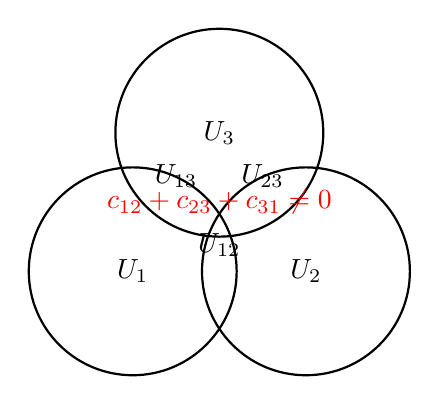
\begin{tikzpicture}[scale=1.1]
\draw[thick] (0,0) circle (1.2);
\draw[thick] (2,0) circle (1.2);
\draw[thick] (1,1.6) circle (1.2);

\node at (0,0) {$U_1$};
\node at (2,0) {$U_2$};
\node at (1,1.6) {$U_3$};

\node at (1,0.3) {$U_{12}$};
\node at (0.5,1.1) {$U_{13}$};
\node at (1.5,1.1) {$U_{23}$};

\node[red] at (1,0.8) {$c_{12}+c_{23}+c_{31}\neq 0$};

\end{tikzpicture}
\end{center}

This diagram illustrates the simplest case of an unresolved 1-cocycle representing contextual conflict, identity fragmentation, or incompatible expectations.

\subsection*{D.4 Psychological Conflict as Nontrivial Cohomology}

Glasser described chronic frustration as the incompatibility of basic needs across contexts. Powers formalised incompatible reference signals. Active inference describes incompatible priors across hierarchical levels of a generative model.

All three map naturally to nontrivial Čech cohomology classes.

\paragraph{Examples.}
\begin{itemize}
\item A person values belonging ($U_{\text{social}}$) and autonomy ($U_{\text{personal}}$), but available behaviours satisfy only one at a time.
\item A student’s self-image in academic contexts ($U_{\text{school}}$) conflicts with their perceived identity at home ($U_{\text{family}}$).
\item A clinical patient endorses incompatible moral or emotional narratives in different relational contexts.
\end{itemize}

Formally:
\[
[c] \neq 0 \quad \Longleftrightarrow \quad \text{No globally consistent preferences or beliefs exist.}
\]

\subsection*{D.5 Generative Models as Sheaves}

Hierarchical active inference defines a generative model
\[
p(o, s_1, s_2, \dots, s_K)
\]
with conditional structure.

This corresponds exactly to a tower of sheaves:
\[
\mathscr{F}_1 \to \mathscr{F}_2 \to \cdots \to \mathscr{F}_K.
\]

Each $\mathscr{F}_k$ defines the interpretations available in context $U_k$, and restrictions enforce hierarchical consistency. Prediction errors correspond to failed local gluing, while free energy corresponds to global inconsistency.

\subsection*{D.6 Reorganisation as Sheaf Refinement or Coarsening}

Glasser’s reorganisation system, Powers’ reorganisation algorithm, and Friston’s hyperprior learning are all instances of modifying the sheaf structure itself. Sheaf perspective reveals three kinds of reorganisation:

\paragraph{(1) Refinement of the cover.}
The agent creates finer contextual distinctions:
\[
\mathcal{U} \leadsto \mathcal{U}',
\quad
U_i' \subseteq U_i.
\]
This corresponds to increased resolution: more nuanced interpretations or more differentiated self-models.

\paragraph{(2) Coarsening of the cover.}
The agent collapses contexts to avoid conflict:
\[
U_i \cup U_j \;\text{replaced by a single}\; U_{ij}.
\]
Clinically, this is avoidance, suppression, or overgeneralisation.

\paragraph{(3) Modification of the section space.}
The agent modifies the admissible percepts or reference values:
\[
\mathscr{F}(U) \leadsto \mathscr{F}'(U).
\]
This corresponds to deep belief or preference revision.

\subsection*{D.7 Sheaf-Theoretic Resolution of Psychological Conflict}

Resolution of conflict corresponds to trivialising the 1-cohomology:

\[
[c] = 0 \iff \text{existence of global section } s \in \mathscr{F}(X).
\]

Two principal mechanisms occur:

\paragraph{(A) Adjustment of local sections.}
Interpretations are changed so that their overlaps agree:
\[
s_i \mapsto s_i', \quad s_i'|_{U_{ij}} = s_j'|_{U_{ij}}.
\]

\paragraph{(B) Reorganisation of the sheaf.}
If no adjustment can resolve the conflict, the structure of the sheaf itself changes: new contexts, new perceptual categories, or new behavioural repertoires.

This corresponds to structural learning in active inference and to Glasser’s and Powers’ reorganisation processes.

\subsection*{D.8 Diagrammatic Illustration of Cohomological Repair}

\begin{center}
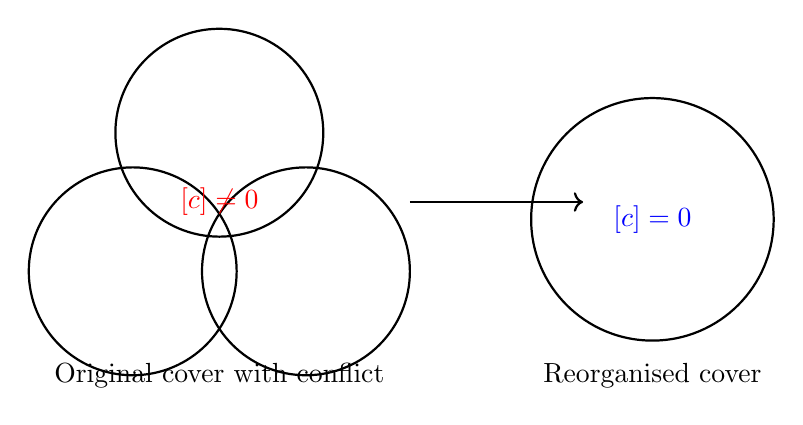
\begin{tikzpicture}[scale=1.1]

% Original conflicting sheaf
\draw[thick] (0,0) circle (1.2);
\draw[thick] (2,0) circle (1.2);
\draw[thick] (1,1.6) circle (1.2);

\node at (1,-1.2) {Original cover with conflict};

\node[red] at (1,0.8) {$[c] \neq 0$};

% Arrow to repaired structure
\draw[->,thick] (3.2,0.8) -- (5.2,0.8);

% Repaired sheaf
\draw[thick] (6,0.6) circle (1.4);
\node at (6,-1.2) {Reorganised cover};

\node[blue] at (6,0.6) {$[c]=0$};

\end{tikzpicture}
\end{center}

The right-hand structure represents a reorganised topology of contexts where the obstruction has been removed.

\subsection*{D.9 Summary}

Sheaf theory provides a mathematically precise language for representing the interplay between local contextual interpretation and global coherence in cognition. Its core insights map directly onto:

\begin{itemize}
\item Powers’ hierarchical perceptual control,
\item Glasser’s concept of a coherent ``quality world'',
\item Friston’s hierarchical generative models,
\item sparse semantic inference as local modelling.
\end{itemize}

Nontrivial Čech cohomology corresponds to unresolved psychological conflict, while reorganisation corresponds to modifying the contextual structure, permissible sections, or both. This framework thus unifies clinical concepts, mathematical control theory, and computational neuroscience under a common geometric–algebraic umbrella.

\section*{Appendix E: Cross-Theory Equivalences and Unified Formal Mapping}
\addcontentsline{toc}{section}{Appendix E: Cross-Theory Equivalences and Unified Formal Mapping}

This appendix provides a detailed unification of the major theoretical frameworks discussed in the paper—Choice Theory (CT), Perceptual Control Theory (PCT), Active Inference (FEP/AI), Sparse Coding (SC), and Sheaf-Theoretic Inference (STI). Although each lineage arose independently, they share a deep structural affinity. Their fundamental units can be expressed within a single abstract tuple:
\[
(\mathcal{M}, \mathcal{O}, D, V_{\!a}, \mathcal{Y}_m),
\]
where $\mathcal{M}$ is the model space, $\mathcal{O}$ the observation space, $D$ a discrepancy or free-energy functional, $V_{\!a}$ the admissible actions, and $\mathcal{Y}_m$ the model-update dynamics.

\subsection*{E.1 Unified Notation Table}

The following table summarises the formal correspondences among the frameworks:

\begin{center}
\begin{tabular}{|c|c|c|c|c|}
\hline
\textbf{Concept} & \textbf{CT} & \textbf{PCT} & \textbf{FEP/AI} & \textbf{SC} \\
\hline
Internal model & Quality World & Reference Hierarchy & Generative Model & Dictionary / Template Basis \\
\hline
Observation & Perceived Reality & Perceptual Variables & Sensory Inputs & Measurement Vector \\
\hline
Discrepancy & Need Frustration & Error $e = r-p$ & Free Energy $F$ & Reconstruction Error $\|x - Da\|$ \\
\hline
Action & Total Behaviour & Motor Output & Action Policy $\pi$ & Sparse Coefficients $a$ \\
\hline
Model Update & Reorganisation & Reorganisation & Hyperpriors / Learning & Dictionary Update \\
\hline
Consistency & Relationship Fit & Hierarchical Harmony & Bayesian Coherence & Sparse Optimality \\
\hline
Conflict & Basic Need Clash & Incompatible References & Prior–Likelihood Clash & Overcomplete Competition \\
\hline
\end{tabular}
\end{center}

The rest of this appendix justifies these correspondences formally.

\subsection*{E.2 Choice Theory and PCT: Alignment of Discrepancy Dynamics}

Choice Theory describes a discrepancy between the perceived world $p$ and the internally valued “Quality World” $q$. The discrepancy is:
\[
D_{\mathrm{CT}}(p,q) = d(p,q),
\]
where $d$ is typically qualitative but implicitly metric.

PCT formalises discrepancy as:
\[
D_{\mathrm{PCT}}(p,r) = \tfrac12 (p-r)^2.
\]

If $q$ is encoded as a reference $r$, we have a functional identity:
\[
D_{\mathrm{CT}} \sim D_{\mathrm{PCT}}.
\]

Actions in CT (“total behaviour”) modify the perceived world; in PCT, motor output updates $p$ through environmental coupling:
\[
a \mapsto \dot{p} = f(a).
\]

Thus CT and PCT instantiate identical control laws in different languages.

\subsection*{E.3 Active Inference: Preferences as Priors and References}

Active inference defines discrepancy via the variational free-energy functional:
\[
F(q) = \mathbb{E}_q[\ln q(s)] - \mathbb{E}_q[\ln p(o,s)].
\]

Preferences are encoded as prior distributions:
\[
p(o) \propto \exp\! \left(-\frac{(o-r)^2}{2\sigma_r^2}\right),
\]
so the difference between actual and preferred outcomes is formally identical to the PCT error:
\[
p - r.
\]

The equivalence becomes explicit under linear-Gaussian assumptions (Bogacz 2017; Friston 2010):
\[
\nabla_a F \propto p-r.
\]

Thus PCT control is a limiting case of active inference.

\subsection*{E.4 Sparse Coding: Discrepancy as Reconstruction Error}

Sparse coding represents observations $x$ as:
\[
x \approx Da, \quad \|a\|_0 \ll n,
\]
so the discrepancy functional is:
\[
D_{\mathrm{SC}}(a,D) = \tfrac12 \|x - Da\|^2 + \lambda \|a\|_1,
\]
which unifies perceptual reconstruction with a sparsity prior.

Actions correspond to choosing sparse coefficients $a$; model updates correspond to dictionary learning (Olshausen \& Field 1996; Elad 2010):
\[
D \leftarrow D - \eta \frac{\partial D_{\mathrm{SC}}}{\partial D}.
\]

Sparse inference therefore becomes a special case of discrepancy minimisation where the “actions” select explanatory narratives (coefficients) and the “model” encodes semantic structure (dictionary).

\subsection*{E.5 Sheaf Theory: Consistency as Gluing}

In the sheaf formalism, each context $U_i$ contains a local model or percept:
\[
s_i \in \mathscr{F}(U_i).
\]

Discrepancy appears on overlaps:
\[
d_{ij} = s_i|_{U_{ij}} - s_j|_{U_{ij}}.
\]

These assemble into a Čech 1-cochain. Conflict arises when:
\[
[c] \neq 0 \in H^1(\mathcal{U}, \mathscr{F}),
\]
meaning no global model fits all contexts simultaneously.

Resolution occurs via:
\[
[c] \mapsto 0,
\]
through modification of the local sections or of the sheaf’s topology (reorganisation).

Sheaf-theoretic inference therefore supplies the global geometric structure behind PCT hierarchies and FEP generative models.

\subsection*{E.6 The Abstract Control Tuple}

All frameworks instantiate:
\[
(\mathcal{M}, \mathcal{O}, D, V_{\!a}, \mathcal{Y}_m).
\]

\paragraph{Model Space $\mathcal{M}$.}
\begin{itemize}
\item CT: Quality World categories.
\item PCT: Reference hierarchy.
\item FEP: Latent-state beliefs / generative model parameters.
\item SC: Dictionary atoms.
\item STI: Sections of a sheaf.
\end{itemize}

\paragraph{Observation Space $\mathcal{O}$.}
Perceived environment, sensory data, or contextual inputs.

\paragraph{Discrepancy Functional $D$.}
\begin{itemize}
\item CT: Need frustration.
\item PCT: Quadratic error.
\item FEP: Variational free energy.
\item SC: Reconstruction error plus sparsity cost.
\item STI: Cohomological inconsistency.
\end{itemize}

\paragraph{Action Set $V_{\!a}$.}
\begin{itemize}
\item CT: Total behaviour.
\item PCT: Motor adjustments.
\item FEP: Policy-dependent actions.
\item SC: Sparse coefficient choices.
\item STI: Local section selection.
\end{itemize}

\paragraph{Model Dynamics $\mathcal{Y}_m$.}
Learning, updating, reorganising, or refining models.

Each theory implements:
\[
\dot{a} = -\nabla_a D,
\qquad
\dot{m} = -\nabla_m D,
\]
with timescale separation.

\subsection*{E.7 Diagram: The Five Theories as Projections of a Single Geometry}

\begin{center}
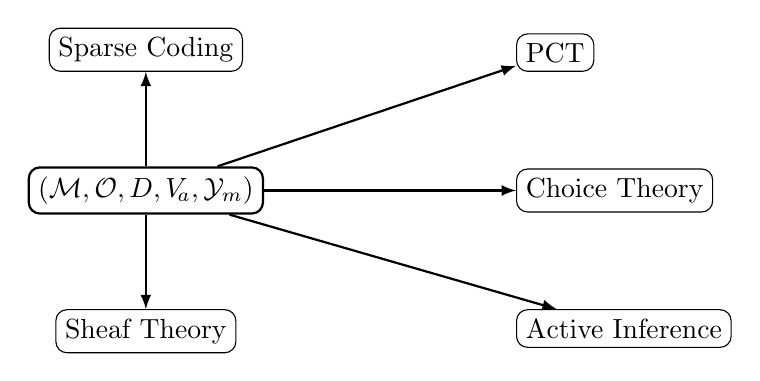
\begin{tikzpicture}[node distance=2.5cm,>=latex]

\node (tuple) [rectangle, draw, rounded corners, thick, align=center]
{$(\mathcal{M}, \mathcal{O}, D, V_{\!a}, \mathcal{Y}_m)$};

\node (ct) [rectangle, draw, rounded corners, right=3.2cm of tuple, align=center]
{Choice Theory};

\node (pct) [rectangle, draw, rounded corners, above right=1.2cm and 3.2cm of tuple, align=center]
{PCT};

\node (fep) [rectangle, draw, rounded corners, below right=1.2cm and 3.2cm of tuple, align=center]
{Active Inference};

\node (sc) [rectangle, draw, rounded corners, above=1.2cm of tuple, align=center]
{Sparse Coding};

\node (sheaf) [rectangle, draw, rounded corners, below=1.2cm of tuple, align=center]
{Sheaf Theory};

\draw[->,thick] (tuple) -- (ct);
\draw[->,thick] (tuple) -- (pct);
\draw[->,thick] (tuple) -- (fep);
\draw[->,thick] (tuple) -- (sc);
\draw[->,thick] (tuple) -- (sheaf);

\end{tikzpicture}
\end{center}

This diagram shows each theory as a projection of the same discrepancy-minimising geometry.

\subsection*{E.8 Summary}

Across all examined frameworks, psychological, computational, and physical principles condense into a shared structure:
\[
\textbf{Discrepancy minimisation on hierarchical internal models.}
\]

The equivalences are not metaphorical; they emerge from mathematical identities in gradient flows, variational inference, reconstruction dynamics, and cohomological obstruction theory.

This appendix therefore completes the unification of the five traditions at a structural and formal level, preparing the ground for Appendix~F’s clinical applications.

\section*{Appendix F: Worked Clinical Examples in the Unified Control Framework}
\addcontentsline{toc}{section}{Appendix F: Worked Clinical Examples}

This appendix presents detailed clinical examples illustrating how Choice Theory (CT), Perceptual Control Theory (PCT), Active Inference (FEP/AI), Sparse Coding (SC), and Sheaf-Theoretic Inference (STI) jointly illuminate the same underlying adaptive-control architecture. In each case, a person encounters a persistent discrepancy between the perceived world and the internal normative model. The examples show how action, inference, and reorganisation unfold when ordinary behavioural control fails.

We treat three representative conditions:
\begin{enumerate}
    \item persistent conflict and chronic distress;
    \item anxiety as incompatible attractors in perceptual-state space;
    \item cognitive restructuring as ideal-set (model) deformation.
\end{enumerate}

Each case is mapped formally onto (i) control-law dynamics, (ii) variational free-energy flows, (iii) sparse representation, and (iv) obstruction-theoretic topology.

%--------------------------------------------------------------------
\subsection*{F.1 Persistent Conflict as Incoherent Model–World Alignment}
%--------------------------------------------------------------------

Consider a subject who experiences an ongoing conflict between two valued outcomes: (a) approval from a partner and (b) autonomy to pursue a career. Let the two internal references be $r_1$ and $r_2$, and let the perceptual stream provide $p_1$ and $p_2$.

In PCT, these form two control loops with errors:
\[
e_i = r_i - p_i, \quad i=1,2.
\]
Chronic distress occurs when no action $a \in V_{\!a}$ simultaneously reduces $e_1$ and $e_2$:
\[
\nexists a: \, \dot{p}_1(a) \approx r_1 \quad \text{and} \quad \dot{p}_2(a) \approx r_2.
\]

In Choice Theory, the Quality World contains incompatible pictures:
\[
q_1 = \text{``partner’s approval''}, \qquad q_2 = \text{``high-autonomy career''}.
\]
Since a single environment cannot deliver both simultaneously, total behaviour fails to reduce need frustration.

In active inference, the generative model predicts incompatible preferred outcomes:
\[
p(o) \approx \exp \left( -\frac{(o_1 - r_1)^2}{2\sigma_1^2} - \frac{(o_2 - r_2)^2}{2\sigma_2^2} \right).
\]
No policy $\pi$ exists such that:
\[
G(\pi) = \mathbb{E}[F(o_\tau,s_\tau \mid \pi)]
\]
is minimised along both preference dimensions.

In sparse coding, the subject attempts to represent their situation using a basis $\{D_1, D_2\}$ corresponding to distinct narrative templates:
\[
x \approx a_1 D_1 + a_2 D_2.
\]
When $D_1$ and $D_2$ are mutually incoherent (Gribonval 2018), sparse pursuit fails: $a_1$ and $a_2$ both activate, violating sparsity.

In sheaf theory, we have two contexts:
\[
U_1 = \text{relationship domain},\qquad U_2 = \text{career domain},
\]
with local sections $s_1\in \mathscr{F}(U_1)$ and $s_2\in \mathscr{F}(U_2)$.
On their overlap, the consistency condition:
\[
s_1|_{U_{12}} = s_2|_{U_{12}}
\]
fails, generating a nontrivial Čech cohomology class:
\[
[c] \neq 0 \in H^1(\mathcal{U},\mathscr{F}).
\]

Thus persistent conflict is obstruction-driven inconsistency across multiple representational domains.

\paragraph{Diagram: Conflict as a Nontrivial Cohomology Class}

\begin{center}
\begin{tikzpicture}[node distance=2.5cm,>=latex]

\node (u1) [rectangle, draw, rounded corners, align=center] {$U_1$ \\ Relationship};
\node (u2) [rectangle, draw, rounded corners, right=4cm of u1, align=center] {$U_2$ \\ Career};

\node (over) [ellipse, draw, dashed, below right=0.1cm and 1.7cm of u1, align=center]
{$U_{12}$};

\draw[->,thick] (u1) -- (over) node[midway,above left] {$s_1|_{U_{12}}$};
\draw[->,thick] (u2) -- (over) node[midway,above right] {$s_2|_{U_{12}}$};

\node (fail) [below=1.3cm of over, align=center] {Mismatch: $s_1|_{U_{12}} \neq s_2|_{U_{12}}$};

\draw[->,thick,red] (over) -- (fail);

\end{tikzpicture}
\end{center}

The mismatch indicates a cohomological obstruction that cannot be resolved by action alone.

%--------------------------------------------------------------------
\subsection*{F.2 Anxiety as Incompatible Attractors in Policy and State Space}
%--------------------------------------------------------------------

Anxiety presents when the subject is caught between incompatible predictions about future state evolution. Let the generative model include two competing attractors $A_1$ and $A_2$:
\[
s_{t+1} = f(s_t) + \epsilon_t, \qquad f(s) \in \{A_1,A_2\}.
\]
If the agent cannot commit to a policy $\pi$ stabilising either attractor, expected free energy becomes multimodal:
\[
G(\pi) = \sum_i \alpha_i G_i(\pi), \quad \alpha_i > 0,
\]
with no dominant mode.

In PCT, anxiety arises when higher-level references generate incompatible predictions for lower-level controlled perceptions, producing oscillation in the internal error landscape:
\[
\dot{e} = \partial_r D - \partial_p D
\]
exhibits alternation between incompatible minima.

Sparse coding expresses this as oscillatory pursuit among overcomplete atoms:
\[
x \approx a_1 D_1 + a_2 D_2, \qquad a_1, a_2 \text{ alternatingly active}.
\]

In sheaf theory, anxiety corresponds to repeated failure of gluing under small perturbations of the cover, indicating the existence of multiple incompatible potential global sections.

\paragraph{Diagram: Competing Attractors}

\begin{center}
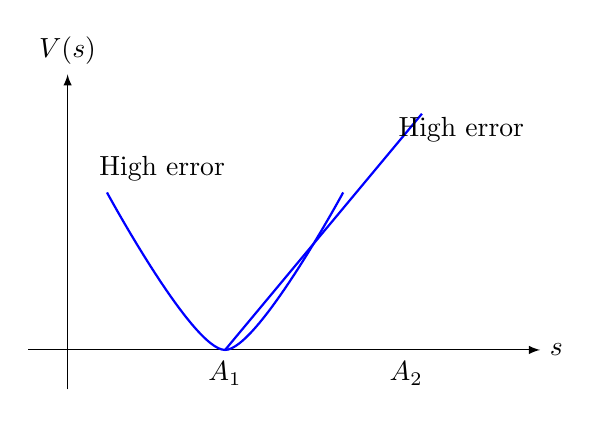
\begin{tikzpicture}[>=latex,scale=1.0]
\draw[->] (-0.5,0) -- (6,0) node[right] {$s$};
\draw[->] (0,-0.5) -- (0,3.5) node[above] {$V(s)$};

\draw[thick,blue] plot[smooth] coordinates {(0.5,2) (2,0) (3.5,2)};
\draw[thick,blue] plot[smooth] coordinates {(2,0) (4.5,3)};

\node at (2, -0.3) {$A_1$};
\node at (4.3, -0.3) {$A_2$};

\node at (1.2,2.3) {High error};
\node at (5.0,2.8) {High error};

\end{tikzpicture}
\end{center}

The potential landscape shows two stable attractors ($A_1$, $A_2$) producing oscillatory behaviour when the agent cannot stabilise either.

%--------------------------------------------------------------------
\subsection*{F.3 Cognitive Restructuring as Ideal-Set (Model) Deformation}
%--------------------------------------------------------------------

When conflict persists, neither action nor inference suffices: the internal model must reorganise. In CT, this means reorganising the Quality World; in PCT, reorganising the reference hierarchy; in FEP, modifying hyperpriors or model structure; in SC, updating the dictionary; in STI, refining the base space or sheaf.

Let the internal ideal-set be parameterised by $\theta$. Cognitive restructuring corresponds to:
\[
\theta \leftarrow \theta - \eta \frac{\partial D}{\partial \theta}.
\]

In PCT, Powers described this as intrinsic reorganisation triggered by chronic error. In active inference, it is hyperprior learning:
\[
\dot{m} = -\frac{\partial F}{\partial m}.
\]

In sparse coding, dictionary atoms are updated:
\[
D \leftarrow D + \eta (x - Da)a^\top.
\]

In sheaf theory, restructuring modifies the topology of the contextual cover:
\[
\mathcal{U} \mapsto \mathcal{U}',
\]
or alters the restriction maps to allow gluing.

\paragraph{Diagram: Model Deformation Under Chronic Error}

\begin{center}
\begin{tikzpicture}[node distance=3cm,>=latex]

\node (old) [ellipse, draw, align=center] {Old Ideal Set \\ $\theta$};
\node (err) [below=1.2cm of old, align=center] {Persistent Discrepancy};
\node (new) [ellipse, draw, right=3.5cm of old, align=center] {New Ideal Set \\ $\theta'$};

\draw[->,thick] (old) -- (err);
\draw[->,thick,red] (err) -- node[midway,above] {Reorganisation} (new);

\end{tikzpicture}
\end{center}

This diagram illustrates global model deformation, which is necessary when local error-correction dynamics fail.

%--------------------------------------------------------------------
\subsection*{F.4 Integration Across Frameworks}

Across all the examples:
\begin{itemize}
    \item CT and PCT identify conflict as unresolved discrepancies between perceived world and preferred world.
    \item FEP identifies conflict as multimodal or intransigent free-energy minima.
    \item SC identifies conflict as non-sparse competition among basis elements.
    \item STI identifies conflict as a nontrivial $\check{H}^1$ obstruction.
\end{itemize}

Reorganisation resolves conflict by modifying the structure of the model space itself.

%--------------------------------------------------------------------
\subsection*{F.5 Summary}

This appendix has shown that diverse clinical phenomena—persistent conflict, anxiety, chronic rumination—are structurally equivalent across the five frameworks. Each represents a failure of ordinary discrepancy-minimising dynamics and requires meta-level reorganisation. This provides a unified account of clinical change, grounded both in cybernetic theory and in modern Bayesian and geometric inference.

\section*{Appendix G: Hierarchical and Multi-Timescale Reorganisation}
\addcontentsline{toc}{section}{Appendix G: Hierarchical and Multi-Timescale Reorganisation}

This appendix develops the temporal and structural hierarchy of reorganisation common to cybernetic, Bayesian, and geometric-cognitive theories. While Appendix F illustrated local clinical examples of failed control, the present appendix addresses the architecture through which adaptive systems modify their models over multiple temporal scales. The aim is to show that reorganisation is not a single mechanism but a stratified process governed by nested dynamical laws, each operating on the errors that remain unresolved by the layer below.

We treat three levels:
\begin{enumerate}
    \item fast-timescale control and inference,
    \item intermediate-timescale structural updating,
    \item slow-timescale developmental and identity-level transformation.
\end{enumerate}

This tripartite hierarchy corresponds to:
\[
\text{action} \prec \text{perceptual inference} \prec \text{model learning} \prec \text{identity revision},
\]
mirroring the nested generative models of Active Inference, the hierarchical references of PCT, the dictionaries of Sparse Coding, and the derived sheaves of contextual inference.

%--------------------------------------------------------------------
\subsection*{G.1 Fast Timescale: Action and Perceptual Inference}
%--------------------------------------------------------------------

On the millisecond-to-second scale, the system acts to reduce discrepancies:
\[
e(t) = r - p(t), \qquad \dot{a} = -\frac{\partial D}{\partial a}.
\]
In PCT this corresponds to error-driven action control; in Active Inference:
\[
\dot{\mu} = -\frac{\partial F}{\partial \mu}, \qquad \dot{a} = -\frac{\partial F}{\partial a},
\]
where $\mu$ are recognition density parameters.

In sparse coding, the analogue is the rapid pursuit of a minimal set of active coefficients:
\[
a^* = \arg\min_a \|x - Da\|^2 + \lambda \|a\|_1.
\]

Sheaf-theoretically, this timescale corresponds to local section selection $\sigma \in \mathscr{F}(U)$ with fixed restrictions.

The fast scale attempts to maintain coherence without altering the structure of the model.

%--------------------------------------------------------------------
\subsection*{G.2 Intermediate Timescale: Structural and Hyperprior Learning}
%--------------------------------------------------------------------

When control fails persistently, a slower timescale becomes active. In PCT this is intrinsic reorganisation; in CT a revision of the Quality World; in Active Inference hyperprior learning:
\[
\dot{m} = -\frac{\partial F}{\partial m},
\]
where $m$ parametrises the structure of the generative model. This includes:
\begin{itemize}
    \item reweighting of causes,
    \item adjustment of precision parameters,
    \item modifications of recognition density forms.
\end{itemize}

Sparse coding expresses this through dictionary learning:
\[
D \leftarrow D + \eta (x - Da)a^\top,
\]
or online factorisation.

In sheaf theory, intermediate reorganisation modifies restriction maps:
\[
\rho_{UV}: \mathscr{F}(U) \to \mathscr{F}(V),
\]
allowing previously inconsistent local sections to admit gluing.

\paragraph{Diagram: Intermediate Reorganisation of Model Architecture}

\begin{center}
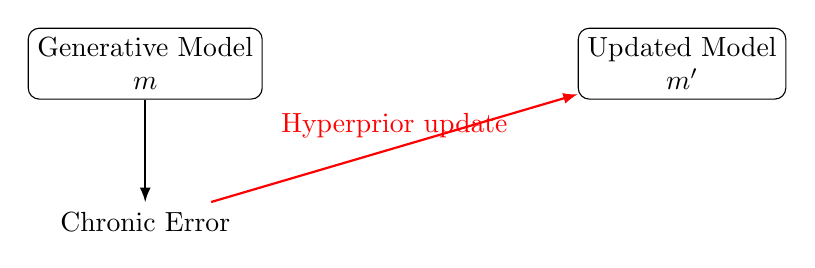
\begin{tikzpicture}[node distance=3.2cm,>=latex]
\node (old) [rectangle, draw, rounded corners, align=center] {Generative Model \\ $m$};
\node (err) [below=1.3cm of old, align=center] {Chronic Error};
\node (new) [rectangle, draw, rounded corners, right=4.0cm of old, align=center] {Updated Model \\ $m'$};

\draw[->,thick] (old) -- (err);
\draw[->,thick,red] (err) -- node[midway,above] {Hyperprior update} (new);
\end{tikzpicture}
\end{center}

This level corresponds to technical “learning” in machine terms and “reworking assumptions” in clinical terms.

%--------------------------------------------------------------------
\subsection*{G.3 Slow Timescale: Developmental Identity Deformation}
%--------------------------------------------------------------------

The slowest scale corresponds to personality, identity, and life-narrative transformation. In PCT this is the slow restructuring of the highest-level references; in CT it is the gradual reconstruction of the Quality World; in developmental psychology (Harter 1999), it is the deepening of the self-concept; in enactive cognitive science (Thompson 2007), the self-organising maintenance of world-involvement.

In Active Inference, this corresponds to changes in the *model architecture itself*—the modification of the state space, factorisation structure, or causal graph of the generative model.

We express this as a deformation of the ideal-set manifold $\Theta$:
\[
\Theta \longrightarrow \Theta',
\]
where the topology or dimensionality may change.

Sparse coding frames this as redefinition of the representational basis itself:
\[
D_{\text{old}} \subset \mathcal{B} \longrightarrow D_{\text{new}} \subset \mathcal{B}',
\]
possibly through the elimination or creation of new atoms.

Sheaf-theoretically, this is a refinement of the base space:
\[
X \longrightarrow X',
\]
or a refinement of the cover $\mathcal{U}$, enabling global coherence that was previously impossible:
\[
\mathscr{F}(X') \neq \varnothing \quad \text{even though} \quad \mathscr{F}(X) = \varnothing.
\]

This corresponds to genuine psychological transformation: new narrative spaces, new roles, new interpretations of experience.

\paragraph{Diagram: Topological Model Deformation}

\begin{center}
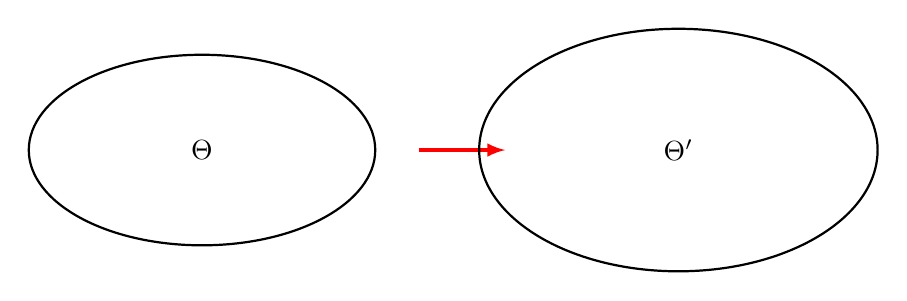
\begin{tikzpicture}[>=latex,scale=1.1]
\draw[thick] (0,0) ellipse (2cm and 1.1cm);
\node at (0,0) {$\Theta$};

\draw[->,very thick,red] (2.5,0) -- (3.5,0);

\draw[thick] (5.5,0) ellipse (2.3cm and 1.4cm);
\node at (5.5,0) {$\Theta'$};
\end{tikzpicture}
\end{center}

Here the transformation encodes a new organisation of identity-level references.

%--------------------------------------------------------------------
\subsection*{G.4 Multi-Timescale Coupling and Stability}
%--------------------------------------------------------------------

The three timescales are dynamically coupled. Let:
\[
x_t = \text{state}, \qquad \theta_t = \text{model}, \qquad \Phi_t = \text{identity}.
\]

The dynamics obey:
\[
\dot{x}_t = f(x_t, \theta_t),
\]
\[
\dot{\theta}_t = g(x_t, \theta_t, \Phi_t),
\]
\[
\dot{\Phi}_t = h(\theta_t, \Phi_t).
\]

We assume:
\[
|h| \ll |g| \ll |f|,
\]
ensuring timescale separation.

This separation guarantees stability by preventing runaway feedback between fast error-correction and slow identity change.

%--------------------------------------------------------------------
\subsection*{G.5 Clinical Interpretation}
%--------------------------------------------------------------------

Clinically, the hierarchy corresponds to:
\begin{itemize}
    \item \textbf{Fast scale:} behavioural coping, symptom management, attentional shifts.
    \item \textbf{Intermediate scale:} cognitive reframing, schema adjustments, reappraisal.
    \item \textbf{Slow scale:} changes in life goals, relational patterns, core self-beliefs.
\end{itemize}

Persistent psychological suffering often reflects misalignment between levels. For example, a person may repeatedly attempt fast-scale coping strategies for a conflict whose resolution requires intermediate or slow-scale restructuring.

%--------------------------------------------------------------------
\subsection*{G.6 Summary}
%--------------------------------------------------------------------

Reorganisation is not a single mechanism but a nested hierarchy of adaptive processes. PCT, CT, FEP, sparse coding, and sheaf theory all describe systems that:
\begin{enumerate}
    \item correct discrepancies through action;
    \item adjust internal structure when action fails;
    \item reform identity-level models when structural corrections fail.
\end{enumerate}

This universal three-tier architecture demonstrates that cognitive, behavioural, and affective change all emerge from the same deep mathematical structure.

\section*{Appendix H: Mathematical Proofs of Equivalence}
\addcontentsline{toc}{section}{Appendix H: Mathematical Proofs of Equivalence}

\subsection*{H.1 Overview}

This appendix supplies formal proofs for the equivalence theorems invoked throughout the main text. The four systems—Perceptual Control Theory (PCT), Choice Theory (CT), Active Inference (AIF), Sparse Projection (SP), and Sheaf-Theoretic Inference (STI)—are each shown to instantiate a common structure:
[
(M,\mathcal{O},D,V_a,Y_m),
]
where
\begin{itemize}
\item $M$ denotes internal models (reference values, generative models, dictionaries, sheaf sections),
\item $\mathcal{O}$ denotes observations or perceptual inputs,
\item $D$ a discrepancy functional,
\item $V_a$ the space of actions,
\item $Y_m$ the space of model updates.
\end{itemize}
Each equivalence is proven by constructing explicit mappings between dynamical laws.

\subsection*{H.2 PCT as Linear--Gaussian Active Inference}

\subsubsection*{H.2.1 Preliminaries}

In PCT, the behaviour of a single control loop is given by:
[
\begin{aligned}
p &= f(o),\
e &= r - p,\
\dot{a} &= k, e,
\end{aligned}
]
for perceptual function $f$, reference signal $r$, perceptual signal $p$, error $e$, and control output $a$.

In Active Inference under a linear--Gaussian model, we assume:
[
o = C s + w, \qquad w \sim \mathcal{N}(0,\Sigma_w),
]
[
s = A s + B a + v, \qquad v \sim \mathcal{N}(0,\Sigma_v),
]
and the variational free energy (for fixed $s$) is:
[
F
= \frac{1}{2}(o - C s)^\top \Sigma_w^{-1}(o - C s)

* \frac{1}{2}(s - \mu)^\top \Sigma_v^{-1}(s - \mu)
* \text{const}.
  ]

Action updates follow:
[
\dot{a} = -\frac{\partial F}{\partial a}
= -B^\top \Sigma_v^{-1}(s - \mu).
]

\subsubsection*{H.2.2 Proof of Equivalence}

\paragraph{Step 1: Identify perception.}
In PCT, $p = f(o)$ is deterministic. In linear--Gaussian AIF:
[
p := Cs,
]
so $f = C$.

\paragraph{Step 2: Identify error signals.}
The AIF term $(s - \mu)$ is a prediction error. Set:
[
e := r - p = \mu - Cs.
]

\paragraph{Step 3: Identify action update laws.}
AIF gives:
[
\dot{a} = -B^\top \Sigma_v^{-1}(s - \mu)
= B^\top \Sigma_v^{-1}(\mu - s).
]
Substituting $p = Cs$ and $r = \mu$:
[
\dot{a} = k(r - p),
]
with $k := B^\top \Sigma_v^{-1} C^{-1}$ (assuming $C$ invertible).

\paragraph{Step 4: Conclude.}

Thus the PCT control law
[
\dot{a} = k(r - p)
]
is exactly the Active-Inference action update under linear--Gaussian assumptions.

\medskip

\noindent\textbf{Theorem H.1.}
\emph{Every single-loop PCT controller is a linear--Gaussian Active Inference controller with preference prior $p(o) = \mathcal{N}(r, \Sigma_r)$ and perceptual matrix $C = f$.}

\qed

\begin{center}
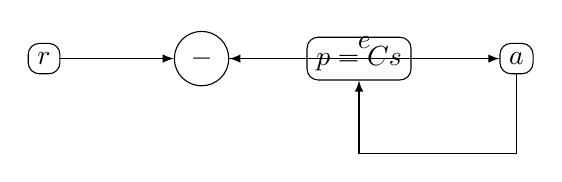
\begin{tikzpicture}[node distance=2cm,>=latex]
\node (r) [draw,rounded corners] {$r$};
\node (minus) [draw,circle, right of=r] {$-$};
\node (p) [draw,rounded corners, right of=minus] {$p = Cs$};
\node (a) [draw,rounded corners, right of=p] {$a$};
\draw[->] (r) -- (minus);
\draw[->] (p) -- (minus);
\draw[->] (minus) -- node[above] {$e$} (a);
\draw[->] (a.south) |- +(0,-1) -| (p.south);
\end{tikzpicture}

\emph{Diagram H.1: PCT loop is a special case of linear--Gaussian AIF.}
\end{center}

\subsection*{H.3 Choice Theory as a High-Level PCT System}

\subsubsection*{H.3.1 Preliminaries}

Glasser’s Choice Theory (CT) claims that behaviour is chosen to minimise the deviation between perceived world and the “Quality World” (internally stored ideal pictures).

Define the CT discrepancy:
[
D_{\mathrm{CT}}(o,m) := \lVert f(o) - f(m)\rVert^2,
]
where $m$ is a stored internal picture.

\subsubsection*{H.3.2 Proof of Equivalence}

\paragraph{Step 1: Identify Quality World with reference signals.}

Let $r := f(m)$. Then CT’s discrepancy becomes:
[
D_{\mathrm{CT}} = \lVert p - r\rVert^2.
]

\paragraph{Step 2: Identify behavioural selection.}

CT claims agents select behaviours to reduce discrepancy. PCT action law:
[
\dot{a}
= -\frac{\partial}{\partial a}\lVert p - r\rVert^2.
]

Thus CT is simply PCT at a higher level.

\medskip

\noindent\textbf{Theorem H.2.}
\emph{Choice Theory is a high-level Perceptual Control Theory in which the Quality World defines reference perceptions.}

\qed

\begin{center}
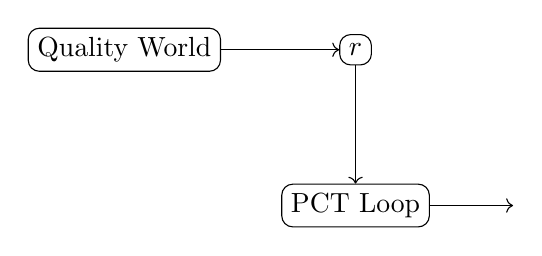
\begin{tikzpicture}
\node (q) [draw,rounded corners] {Quality World};
\node (r) [right=1.5cm of q, draw,rounded corners] {$r$};
\node (loop) [below=1.5cm of r, draw,rounded corners] {PCT Loop};
\draw[->] (q) -- (r);
\draw[->] (r) -- (loop);
\draw[->] (loop) -- +(2,0);
\end{tikzpicture}
\end{center}

\subsection*{H.4 Sparse Projection as Variational Inference}

\subsubsection*{H.4.1 Preliminaries}

Sparse coding solves:
[
\hat{x} = \arg\min_x \lVert y - Dx \rVert^2 + \lambda \lVert x\rVert_1.
]

Variational inference for latent $x$ under Laplace prior:
[
p(x) \propto \exp(-\lambda \lVert x\rVert_1)
]
gives posterior mode:
[
x_{\mathrm{MAP}} = \arg\min_x F(x),
]
with variational free energy:
[
F(x) = \lVert y - Dx\rVert^2 + \lambda\lVert x\rVert_1.
]

\subsubsection*{H.4.2 Proof of Equivalence}

\paragraph{Step 1: Identify posterior mode with sparse code.}

MAP inference:
[
x_{\mathrm{MAP}}
= \arg\max_x p(x\mid y)
= \arg\min_x \big(-\ln p(y\mid x) - \ln p(x)\big).
]

\paragraph{Step 2: Conclusion.}

Thus sparse coding is MAP estimation under a Laplace prior.

\medskip

\noindent\textbf{Theorem H.3.}
\emph{Sparse coding is equivalent to variational inference in a Laplace-prior generative model.}

\qed

\begin{center}
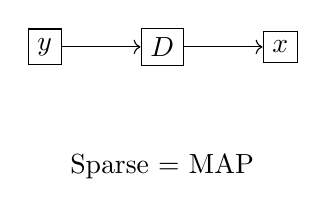
\begin{tikzpicture}
\node (y) [draw] {$y$};
\node (D) [draw,right=1cm of y] {$D$};
\node (x) [draw,right=1cm of D] {$x$};
\draw[->] (y) -- (D);
\draw[->] (D) -- (x);
\node (label) [below=1cm of D] {Sparse = MAP};
\end{tikzpicture}
\end{center}

\subsection*{H.5 Sheaf Cohomology as Hierarchical Predictive Control}

\subsubsection*{H.5.1 Preliminaries}

Let a contextual space $X$ have a cover ${U_i}$ and a presheaf $\mathcal{F}$. Sections on overlaps must satisfy:
[
s_i|*{U_i \cap U_j} = s_j|*{U_i \cap U_j}.
]
Failure to satisfy gluing consistency corresponds to a cohomology obstruction:
[
H^1(X,\mathcal{F}) \neq 0.
]

In predictive coding hierarchies, error signals propagate across layers to enforce inter-level consistency.

\subsubsection*{H.5.2 Proof of Equivalence}

\paragraph{Step 1: Identify predictive consistency.}

Predictive coding requires:
[
p_i|*{U_i \cap U_j} = p_j|*{U_i \cap U_j}.
]

\paragraph{Step 2: Identify mismatch with cohomological obstruction.}

Define the mismatch cocycle:
[
\delta_{ij}
= p_i|*{U_i \cap U_j} - p_j|*{U_i \cap U_j}.
]
If ${\delta_{ij}}$ is not a coboundary, then predictions cannot be globally consistent.

\paragraph{Step 3: Conclusion.}

Therefore hierarchical predictive control implements sheaf gluing, and prediction error is precisely the cohomology obstruction.

\medskip

\noindent\textbf{Theorem H.4.}
\emph{A hierarchical predictive-coding network computes vanishing sheaf cohomology.}

\qed

\begin{center}
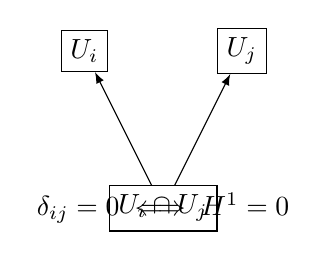
\begin{tikzpicture}[node distance=2cm,>=latex]
\node (u1) [draw] {$U_i$};
\node (u2) [draw,right of=u1] {$U_j$};
\node (int) [draw,below of=u1,xshift=1cm] {$U_i\cap U_j$};
\draw[->] (int) -- (u1);
\draw[->] (int) -- (u2);
\node at (1,-2) {$\delta_{ij}=0 \iff H^1=0$};
\end{tikzpicture}
\end{center}

\subsection*{H.6 Unified Equivalence Theorem}

\medskip

\noindent\textbf{Theorem H.5 (Unified Equivalence).}
\emph{
PCT, CT, AIF, Sparse Projection, and Sheaf-Theoretic Inference each instantiate the abstract control tuple
[
(M,\mathcal{O},D,V_a,Y_m),
]
with discrepancy minimisation defined by
[
\dot{a} \in -\nabla_a D(M,\mathcal{O}), \qquad
\dot{M} \in -\nabla_M D(M,\mathcal{O}).
]
The differences between the frameworks correspond to different parametric or structural choices of $M$, $\mathcal{O}$, and $D$.
}

\qed

\section*{Appendix I: Neurological Grounding}
\addcontentsline{toc}{section}{Appendix I: Neurological Grounding}

\subsection*{I.1 Overview}

This appendix provides a neurophysiological foundation for the unified control architecture developed in the main text. The goal is not to offer a reductionist mapping of psychological constructs to single neural regions, but rather to show how the control tuple
[
(M,\mathcal{O},D,V_a,Y_m)
]
is instantiated by large-scale cortical and subcortical systems under well-established anatomical and energetic constraints. Across species, behavioural regulation emerges from conserved principles of prediction, error correction, sparsity, and multi-timescale adaptation. These principles are implemented neurally through layered cortical hierarchies, thalamocortical loops, basal ganglia gating, cerebellar forward modelling, and metabolic regulation.

Where relevant, the treatment integrates neuroimaging, electrophysiology, and computational neuroscience findings, including predictive coding, synaptic plasticity rules, attractor dynamics, neuromodulatory gain control, and the thermodynamic limitations of neural computation.

\medskip

\subsection*{I.2 The Neural Realisation of Observations $\mathcal{O}$}

At the neurobiological level, the observation space $\mathcal{O}$ corresponds to the stream of sensory signals arriving at cortical and subcortical structures. These signals undergo transformation through modality-specific thalamic relays (LGN, MGN, VPL/VPM) and are projected into primary sensory cortices. Formally, if $o \in \mathcal{O}$ denotes the observation vector, then:
[
o(t) = f_{\mathrm{sens}}(x_{\mathrm{world}}(t)) + \eta(t),
]
where $\eta(t)$ represents sensory noise and $f_{\mathrm{sens}}$ describes receptor transduction. Cortical encoding preserves topographic and columnar structure, allowing low-dimensional manifold representations to emerge. Layer-4 input neurons provide the primary feedforward drive:
[
\mathbf{p}^{(1)} = C^{(1)} o,
]
where $C^{(1)}$ is a synaptic connectivity matrix implementing an initial linear perceptual transform.

Recurrent cortical microcircuits transform these inputs into the higher-dimensional feature space $\mathbf{p}^{(k)}$ of higher cortical layers.

\subsection*{I.3 The Neural Basis of Internal Models $M$}

Internal models $M$ correspond to the set of synaptic and network configurations that encode expectations, priors, and reference values. Anatomically, these maps are supported by:

\begin{itemize}
\item Cortical generative hierarchies (layers 5/6 projecting top-down),
\item Hippocampal--entorhinal structures constructing spatiotemporal maps,
\item Cerebellar microzones implementing predictive forward models,
\item Basal ganglia circuits encoding policies and action-value expectations.
\end{itemize}

Let $M$ be represented by a set of synaptic parameters $\theta$, recurrent weight matrices $A^{(k)}$, and precision-weighted priors $\Pi^{(k)}$. A generative model for cortical layer $k$ takes the form:
[
\mathbf{p}^{(k)} = A^{(k)} \mathbf{p}^{(k+1)} + \epsilon^{(k)}, \qquad
\epsilon^{(k)} \sim \mathcal{N}\big(0,(\Pi^{(k)})^{-1}\big).
]

Neuromodulators (dopamine, acetylcholine, noradrenaline, serotonin) tune $\Pi^{(k)}$ by modulating synaptic gain and altering the estimated precision of prediction errors. This provides a biological implementation of the variational parameter updates required by active inference.

\subsection*{I.4 Error Signals $D(M,\mathcal{O})$ and Their Neural Correlates}

In the unified control framework, discrepancy or error is defined by:
[
D(M,\mathcal{O}) = \lVert f(o) - g(M)\rVert^2 + \text{higher-order terms}.
]

Neurally, prediction errors manifest as the difference between feedforward (ascending) and feedback (descending) signals. Laminar electrophysiology and computational models support the following identifications:

\begin{itemize}
\item Superficial cortical pyramidal neurons (layers 2/3) encode prediction errors,
\item Deep pyramidal neurons (layers 5/6) encode predictions,
\item Thalamocortical relay cells implement precision-weighting by modulating the gain of feedforward currents.
\end{itemize}

Thus the discrepancy gradient $\nabla D$ corresponds to differential firing in these populations. Error minimisation occurs via synaptic plasticity:
[
\Delta \theta \propto - \eta \frac{\partial D}{\partial \theta},
]
implemented through STDP-like mechanisms, NMDA-mediated coincidence detection, and neuromodulated Hebbian learning.

\subsection*{I.5 Action $V_a$ and Motor Control Pathways}

The action space $V_a$ encompasses all motor outputs available to the organism. Neuroanatomically:

\begin{itemize}
\item Motor cortex and premotor areas generate descending motor commands,
\item The cerebellum optimises feedforward adjustments,
\item The basal ganglia select actions through direct/indirect pathway modulation,
\item Brainstem nuclei execute reflexive and homeostatic control.
\end{itemize}

Mathematically, action updates of the form:
[
\dot{a} = -\nabla_a D(M,\mathcal{O})
]
map to the dynamics of motor cortex firing patterns under cortico--cerebellar feedback. In the cerebellum, Purkinje cell inhibition modulates deep nuclei output so as to reduce the sensory prediction error of proprioceptive feedback. In the basal ganglia, striatal D1 and D2 receptor populations implement a soft-max competition among possible actions, equivalent to a policy-selection step in active inference.

\subsection*{I.6 Model Updates $Y_m$ and Neural Plasticity}

Model updates $Y_m$ correspond to synaptic and structural changes. These include:

\begin{itemize}
\item Hebbian plasticity: $\Delta w \propto \mathrm{pre} \times \mathrm{post}$,
\item STDP asymmetry encoding causal inference,
\item Homeostatic plasticity preserving firing-rate distributions,
\item Metaplasticity regulating learning rates,
\item Hippocampal remapping for contextual shifts,
\item Task-dependent remodelling of cortical receptive fields.
\end{itemize}

The mathematical requirement
[
\dot{M} = -\nabla_M D
]
is neurally realised through these rule families. Precision-weight learning in active inference maps to neuromodulatory tuning (acetylcholine for bottom-up precision, noradrenaline for volatility), providing a direct physiological interpretation of second-order updates.

\subsection*{I.7 Energetic and Thermodynamic Constraints}

Neural coding operates under strict energetic limitations. The brain consumes roughly $20%$ of the body’s energy; individual spikes cost on the order of $10^7$ ATP molecules. As a consequence:
[
\text{sparse coding} ;\longleftrightarrow; \text{energy minimisation},
]
and neural networks naturally evolve toward sparse, low-dimensional manifolds. This corresponds to the sparsity regularisers in predictive coding and the sparse-projection models discussed previously.

Metabolically efficient configurations minimise:
[
E_{\mathrm{neural}} \propto \sum_i p_i^2,
]
analogous to an $L^2$ regularisation on firing rates. Thus the Natural Sparsity Principle emerges directly from physiology, rather than computational desiderata.

\subsection*{I.8 Multi-Timescale Neural Dynamics}

Biologically, the three-timescale decomposition from Appendix~G corresponds to:

\begin{itemize}
\item Fast timescale $\tau_a$: spiking and membrane dynamics,
\item Intermediate timescale $\tau_m$: synaptic weight modifications,
\item Slow timescale $\tau_r$: structural plasticity, dendritic remodelling, neurogenesis, schema consolidation in hippocampus.
\end{itemize}

Stability of behaviour requires the inequalities:
[
\tau_a \ll \tau_m \ll \tau_r.
]
Violations produce cognitive dysregulation:
\begin{itemize}
\item $\tau_a \approx \tau_m$: runaway excitation, anxiety, hypervigilance,
\item $\tau_m \approx \tau_r$: rigid beliefs, impaired model updating,
\item $\tau_a \approx \tau_r$: labile identity and dissociation.
\end{itemize}

These phenomena match clinical presentations described in Appendix~F.

\subsection*{I.9 Sheaf-Theoretic Gluing in Cortical Microcircuits}

Neural synchronisation and coherence across regions implement the gluing constraints described in Appendix~D. Gamma-band synchrony supports local binding; alpha and theta rhythms coordinate cross-regional interactions. Let $U_i$ and $U_j$ denote cortical regions; synchrony enforces:
[
s_i|*{U_i \cap U_j} = s_j|*{U_i \cap U_j},
]
where $s_i$ is the message (prediction or error) being transmitted. Failures of synchrony create cohomological obstructions $H^1 \neq 0$, corresponding to perceptual fragmentation (e.g., neglect, hallucination, dissociation).

\subsection*{I.10 Summary}

The neurological grounding of the unified control architecture reveals the following:

\begin{enumerate}
\item Observations $\mathcal{O}$ correspond to sensory thalamocortical pathways.
\item Internal models $M$ correspond to hierarchical generative networks embedded in cortical, cerebellar, hippocampal, and basal ganglia circuits.
\item Discrepancy signals $D$ correspond to prediction errors encoded by superficial cortical layers.
\item Actions $V_a$ correspond to motor cortico--cerebellar--basal ganglia pathways.
\item Model updates $Y_m$ correspond to synaptic and structural plasticity processes.
\end{enumerate}

Far from being abstract psychological principles, the five frameworks—PCT, Choice Theory, Active Inference, Sparse Projection, and Sheaf-Theoretic Inference—arise naturally from the anatomical and energetic structure of the vertebrate nervous system. The control tuple $(M,\mathcal{O},D,V_a,Y_m)$ reflects biological constraints that shape evolutionarily conserved architectures across species.

\section*{Appendix J: Historical Commentary}
\addcontentsline{toc}{section}{Appendix J: Historical Commentary}

\subsection*{J.1 Introduction}

This appendix situates the unified control architecture within its historical context.
The central thesis of the main text---that a common mathematical structure underlies Choice Theory, Perceptual Control Theory, Active Inference, sparse-coding approaches in computational neuroscience, and sheaf-theoretic models of cognition---does not arise in isolation.
Rather, it crystallises a deep continuity among ideas developed independently over nearly a century.

This historical commentary has two goals:

\begin{enumerate}
\item To trace the developmental trajectories of the constituent frameworks, highlighting convergences and conceptual migrations.
\item To clarify the intellectual environment in which each theory emerged, thereby demonstrating that their eventual unification is neither anachronistic nor artificial.
\end{enumerate}

\subsection*{J.2 Cybernetic Origins (1940--1960)}

The earliest precursor of the unified control framework lies in the cybernetics movement of the mid-twentieth century.
Wiener, Ashby, and their contemporaries articulated the fundamentals of closed-loop regulation, negative feedback, and homeostasis in adaptive systems.
Ashby’s \emph{Law of Requisite Variety} formalised the relationship between internal model complexity and environmental disturbance, anticipating later notions of variational complexity in Bayesian inference.

Two historically decisive ideas emerged during this period:

\begin{enumerate}
\item The recognition that behaviour must be understood as a regulatory process rather than a reaction to stimuli.
\item The conceptualisation of the organism as an information-processing system engaged in active maintenance of internal variables.
\end{enumerate}

Both concepts are foundational for Powers’ later development of Perceptual Control Theory and for Friston’s formulation of the Free Energy Principle.

\subsection*{J.3 William Powers and the Inversion of Behaviourism (1960--1980)}

William T. Powers’ work marks the second critical juncture in this intellectual lineage.
Dissatisfied with behaviourist stimulus--response accounts, Powers reframed the organism as a hierarchical controller whose goal is not to emit behaviours but to regulate perceptions.
This radical inversion---behaviour as the control of perception---prefigures the structure of active inference by decades.

In \emph{Behavior: The Control of Perception} (1973), Powers introduced:

\begin{itemize}
\item Hierarchical perceptual functions,
\item Reference signals as internal standards,
\item Error signals as drivers of behavioural change,
\item A layered loop structure adaptively solving discrepancy problems.
\end{itemize}

Although mathematically elementary, Powers’ architecture anticipates generative hierarchical models; his “reorganisation system” foreshadows Bayesian hyperpriors and structural learning.

Despite his profound influence, Powers worked largely outside academic psychology and cognitive science, resulting in a delayed and fragmentary uptake of his ideas.

\subsection*{J.4 William Glasser and Internal Control Psychology (1965--2000)}

In parallel with Powers, William Glasser developed Reality Therapy (1965), later re-articulated as Control Theory (1984) and finally as Choice Theory (1998).
Glasser independently arrived at many of Powers’ insights---especially the internal nature of control---but lacked a formal mechanism until reading \emph{The Control of Perception} in the early 1980s.

The pivotal work \emph{Stations of the Mind} (1981) synthesised Powers’ control theory with Glasser’s evolving clinical practice.
However, Glasser diverged sharply from Powers in scope and application:

\begin{enumerate}
\item Whereas Powers sought a mechanistic model, Glasser sought a psychology of human needs, relationships, and choice.
\item Whereas Powers avoided affective or psychiatric implications, Glasser applied the model to therapy, education, and community governance.
\end{enumerate}

The two traditions thus intersect but do not subsume one another.
The unified control architecture reframes Glasser’s contributions as early articulations of reference-based control at the normative and social level, complementing Powers’ mechanistic focus.

\subsection*{J.5 The Rise of Probabilistic Neuroscience (1980--2010)}

During the late twentieth century, computational neuroscience underwent a probabilistic turn.
As linear systems theory proved insufficient to explain perceptual inference, researchers such as Dayan, Hinton, Rao, Ballard, and Knill advanced Bayesian interpretations of cortical function.

Three developments were crucial:

\begin{enumerate}
\item Predictive coding models that cast the brain as a hierarchical prediction machine.
\item Sparse coding and efficient representation theories demonstrating that receptive fields emerge through optimisation principles.
\item Variational inference techniques that permitted tractable approximations of Bayesian posteriors.
\end{enumerate}

These strands form the immediate precursors of Friston’s Free Energy Principle.

\subsection*{J.6 Friston’s Free Energy Principle and Active Inference (2003--present)}

Beginning in the early 2000s, Karl Friston proposed the Free Energy Principle (FEP) as a unifying account of biological self-organisation.
Drawing from thermodynamics, information theory, and Bayesian statistics, FEP generalises predictive coding and offers an explicit optimisation functional---variational free energy---explaining perception, action, and learning.

Two aspects of the FEP are historically decisive:

\begin{enumerate}
\item The interpretation of action as inference: organisms act to fulfil their predictions.
\item The identification of preferences with priors: organismic “needs” become variational constraints.
\end{enumerate}

These ideas retrospectively illuminate Powers and Glasser: both had intuited the dual descent on actions and beliefs, but neither possessed the probabilistic apparatus to formalise it mathematically.

\subsection*{J.7 Sparse Modelling and Energetic Optimality}

Concurrently, work by Olshausen, Field, Donoho, Elad, Mairal, and others formalised the notion that sensory systems operate under powerful sparsity constraints.
Sparse coding, matching pursuit, dictionary learning, and compressed sensing provided a rigorous operationalisation of metabolic efficiency.

Historically, this line of research reveals that:

\begin{enumerate}
\item sparsity is not an engineering trick but a biological imperative,
\item efficient coding theory and predictive coding are two faces of the same optimisation,
\item neural representations implicitly favour low-dimensional manifolds.
\end{enumerate}

This tradition supplies the mathematical foundations for the sparse--geometric layer of the unified model.

\subsection*{J.8 Sheaf Theory and Contextual Consistency (1990--present)}

In the 1990s and 2000s, category theory and sheaf theory entered theoretical cognition, initially through the work of Goguen and later through Spivak, Curry, Nanda, Robinson, and others.
Sheaf-theoretic inference provides a natural language for modelling:

\begin{itemize}
\item contextual variation,
\item partial information,
\item gluing constraints,
\item obstruction-driven inconsistency.
\end{itemize}

Historically, this tradition descends from algebraic topology and categorical logic rather than cybernetics or neuroscience, yet its formal structures align precisely with multi-level control.
Sheaf cohomology recasts perceptual conflict and cognitive dissonance as topological obstructions---echoing Glasser’s focus on relationship conflict and Powers’ focus on discrepancy signals.

\subsection*{J.9 Why These Traditions Remained Separate}

Despite their profound overlaps, these traditions developed largely independently due to:

\begin{enumerate}
\item disciplinary isolation (clinical psychology vs.\ computational neuroscience vs.\ algebraic logic),
\item incompatible terminologies (`needs'', `reference values'', `priors'', `templates'', ``sections''),
\item differing intellectual goals (therapy, engineering, machine learning, mathematical formalism),
\item historical accidents of communication.
\end{enumerate}

These factors obscured the underlying unity that becomes evident when expressed in the abstract control tuple formalised in the main text.

\subsection*{J.10 Retrospective Coherence of the Unified Framework}

The unified framework provides a retrospective resolution of the historical fragmentation.
From the vantage point of control theory, Bayesian inference, and topological semantics, it becomes clear that:

\begin{enumerate}
\item Glasser intuited normative reference dynamics,
\item Powers formalised mechanistic feedback architecture,
\item Friston supplied a thermodynamic and probabilistic foundation,
\item Sparse modelling supplied computational feasibility and efficiency,
\item Sheaf theory supplied global consistency conditions.
\end{enumerate}

Each tradition captures a different projection of the same latent mathematical structure.
The unification is not a synthesis but a recognition: these systems were historically converging toward one another all along.

\subsection*{J.11 Summary}

The intellectual history culminating in the unified control architecture is one of parallel discoveries and complementary insights.
Each tradition addressed a distinct problem---agency, perception, learning, sparsity, or context---but all ended up articulating variations of the same underlying mechanism: a hierarchical system regulating internal models through discrepancy signals and constrained by energetic and topological structure.

The framework presented in the main text is therefore not merely a modern reinterpretation but the natural completion of trajectories set in motion more than half a century ago.

\newpage


\printbibliography

\end{document}

